%%%%%%%%%%%% BASES DE DATOS %%%%%%%%%%%%%%%%%%%%%
\chapter{Bases de datos}\label{ch:BBDDs}

\begin{table}[ht!]
     \centering
     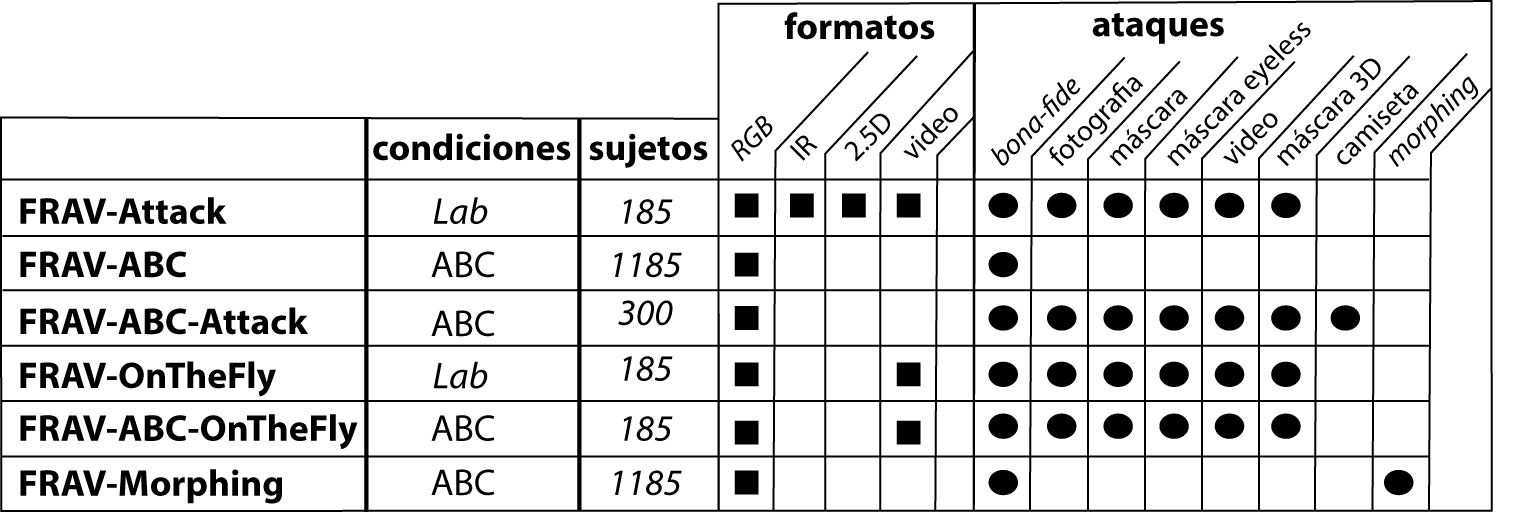
\includegraphics[width=1\textwidth]{ch-sistemasABC/images/ch-BBDDs/TABLA_BASES_DE_DATOS.png}
     \caption{Bases de datos para la detección de ataques de presentación en sistemas \GLS{ABC}.}
     \label{tab:TablaBasesDatos}
\end{table}

En cada una de las secciones de este capítulo se describen las características de las bases de datos construidas para llevar a cabo las investigaciones expuestas a lo largo de los siguientes capítulos. En la tabla \ref{tab:TablaBasesDatos} se pueden ver algunas características de cada una de estas bases de datos: número de sujetos, ataques de presentación considerados y dispositivo o dispositivos empleados para su captura.

En la sección \ref{sec:BBDD-FRAV-Attack} se presenta \Gls{FRAV-Attack}, una base de datos con ataques de presentación llevados a cabo con distintos artefactos y capturados con diferentes tipos de sensores. Con esta base de datos, capturada en laboratorio, se ha entrenamiento el método \GLS{PAD} descrito en el capitulo \ref{ch:PAD_MULTIATAQUE} y que se puso a prueba en condiciones reales en los experimentos descritos en el capitulo \ref{ch:EVALUACIONACION_TOPOLOGIAS}. 


A continuación, en la sección \ref{sec:BBDD-ABC} se presentan dos bases de datos capturadas en dispositivos \GLS{ABC} operativos, en cruces de frontera reales: \Gls{FRAV-ABC} con imágenes \textit{<<\gls{chip}>>} de pasaportes e imágenes \gls{vivo} capturadas en el propio dispositivo y \Gls{FRAV-ABC-Attack} con los mimos tipos de imágenes pero que además incluye ataques de presentación en las imágenes \gls{vivo}.

En la sección \ref{sec:BBDD-OnTheFly} se describen otras dos bases de datos construidas para el la publicación \cite{ortega2020dynamic}, que se detalla en el capítulo \ref{fig:EsquemaCapturaFRAVABCOmTheFly}. Por un lado la base de datos \Gls{FRAV-OnTheFly} capturada en un laboratorio, en condiciones controladas, simulando el comportamiento de viajeros frente a un sistema \GLS{ABC} con captura dinámica (para mas información sobre este tipo de sistemas \GLS{ABC}. ver apartado \ref{subsec:ArquitecturaFisicaABC}). Y por otro lado, las base de datos \Gls{FRAV-ABC-OnTheFly}, capturada en \GLS{ABC} con captura dinámica, en un cruce de fronteras real.

La sección \ref{sec:BBDD_Morphing} describe la base de datos, \gls{FRAV-Morphing}, construida a partir de \GLS{FRAV-ABC} para la investigación publicada sobre ataques de \gls{morphing} en sistemas \GLS{ABC} \cite{ortega2020border} que se presenta en detalle en el capitulo \ref{ch:morphing}. Además de describir la estructura de la base de datos también se detalla cómo se construyeron las imágenes con los ataques \gls{morphing}.


%%%%%%%%%%%%%% FRAV ATTACK    %%%%%%%%%%%%%%%%%%%%%%%%%%%%%%
\section{FRAV-Attack: Base de datos multimodal de ataques biométricos}\label{sec:BBDD-FRAV-Attack}

\begin{figure}[t!]
\centering
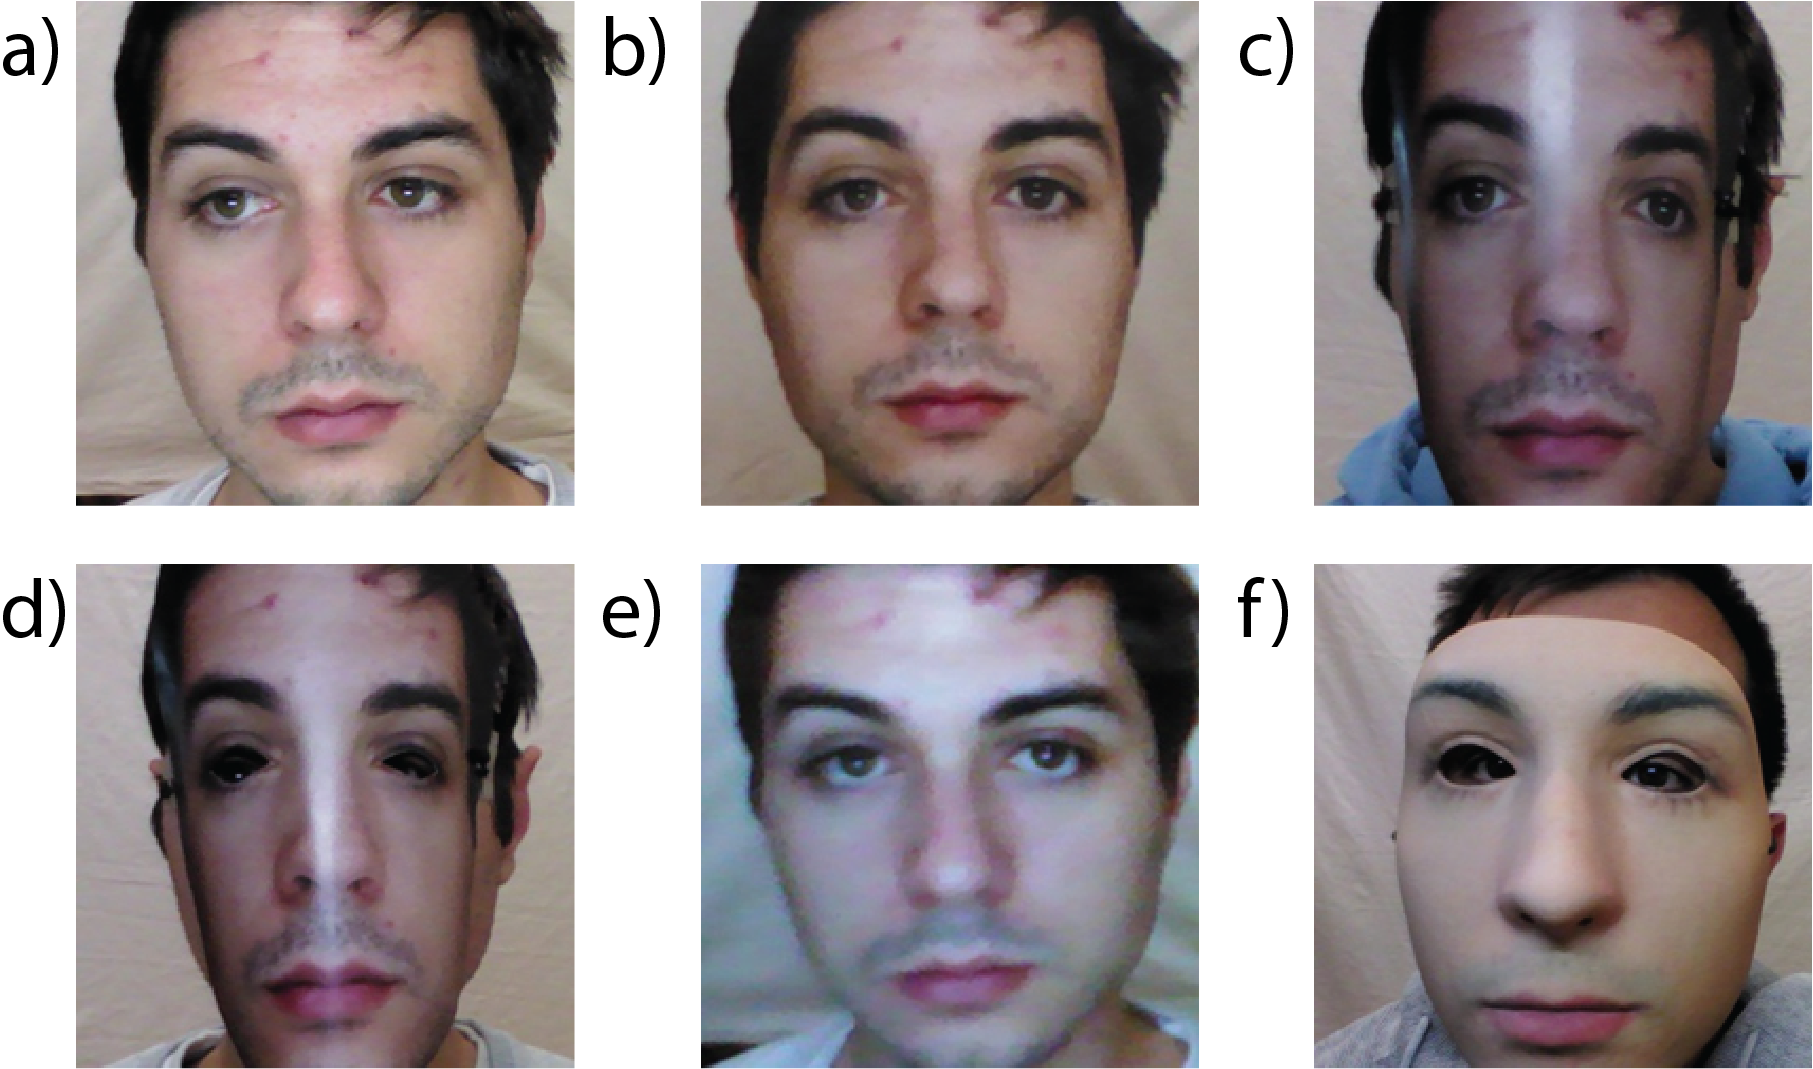
\includegraphics[width=1\textwidth]{ch-sistemasABC/images/ch-BBDDs/ATAQUES.png}
    \caption{Capturas \gls{bona-fide} y distintos ataques con la identidad de un mismo sujeto en \Gls{FRAV-Attack}. (a) \gls{bona-fide}, (b) \GLS{PAI} fotografía, (c) \GLS{PAI} máscara de cartón, (d) \GLS{PAI} máscara de cartón  sin ojos, (e)  \GLS{PAI} video y (f) \GLS{PAI} máscara $3$D.}
    \label{fig:DISTINTOS_ATAQUES_EN_FRAV_ATTACK}
\end{figure}

Aunque existe un gran número de publicaciones sobre detección de ataques de presentación, habitualmente tienen en cuenta pocos tipos de ataques diferentes y utilizan un único tipo de sensor para realizar las captura. \Gls{FRAV-Attack} se construyo con el objetivo de implementar y evaluar un método \GLS{PAD} multi-ataque y multi-sensor como el que se presenta en el Capitulo \ref{ch:PAD_MULTIATAQUE}. La base de datos incluye diferentes tipos de ataque y capturas realizadas con distintos tipos de sensores.

\begin{figure}[ht]
     \centering
     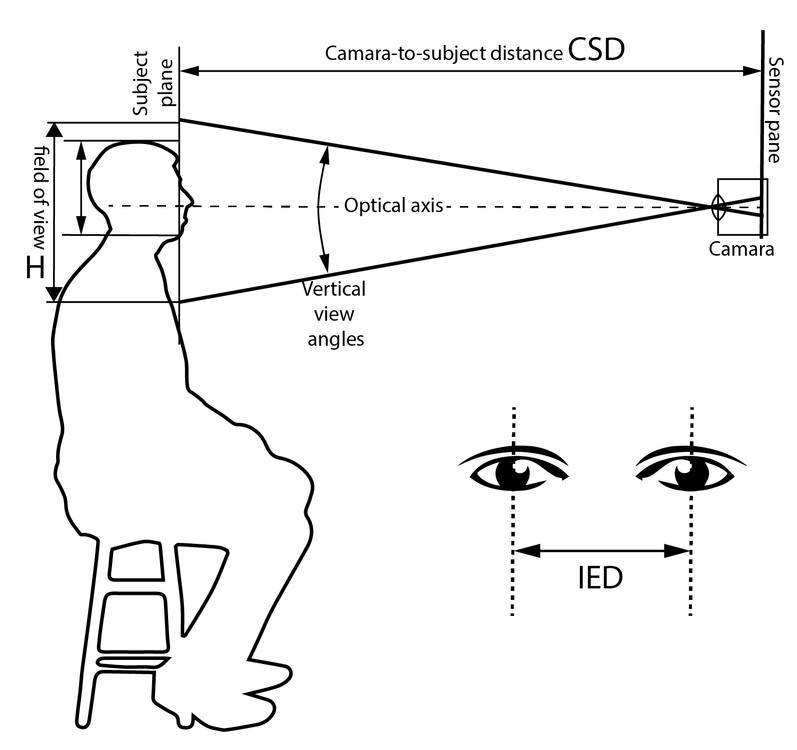
\includegraphics[width=0.6\textwidth]{ch-sistemasABC/images/ch-BBDDs/CAPTURA_ESTATICA.png}
     \caption{Esquema del proceso de captura de \Gls{FRAV-Attack}.}
     \label{fig:EsquemaCapturaFRAVAttack}
\end{figure}

La base de datos fue capturada por el grupo de investigación \GLS{FRAV} en un laboratorio de la universidad \GLS{URJC} bajo condiciones controlados de iluminación, de fondo y de pose. Para la iluminación se usaron dos tipos de iluminación en cada captura: luz halógena y luz infrarroja \GLS{IR}. Y de cada sujeto se capturaron tres poses: frontal, lateral derecha y lateral izquierda. La pose frontal cumple las normas fijadas en el estándar de \GLS{ICAO} Doc $9303$ \cite{doc20069303}) para documentos de viaje (ver Fig.\ref{fig:EsquemaCapturaFRAVAttack}), que recomienda una distancia al sensor \GLS{CSD} y una distancia intraocular \GLS{IED} (ver Tabla \ref{tab:distanciasICAO}).   

Entre los sujetos de la base de datos se incluyeron, tanto estudiantes como personal docente y de servicios de la propia universidad buscando una muestra lo más heterogénea posible. Finalmente la base de datos contiene 185 sujetos, 88 mujeres y 97 hombres, de edades comprendidas entre los 18 y los 53 años. Las capturas de un mismo sujeto se realizaron en una única sesión.

\begin{table}[t!]
    \centering
    \begin{tabular}{|l|c|c|} \hline
    \multicolumn{1}{|p{2cm}|}{} & \multicolumn{1}{|p{4cm}|}{\centering\textbf{IEC}} & \multicolumn{1}{|p{5cm}|}{\centering\textbf{CSD}} \\ \hline 
    \small{\textbf{Requerido}} & \textbf{IEC} $\geq 90$ mm  & $0.7 m\leq $ \textbf{CSD} $\leq 4$ m\\ \hline  \small{\textbf{Recomendado}} & \textbf{IEC} $\geq 120$ mm. & $1 m\leq $ \textbf{CSD} $\leq 2.5$ m\\ \hline 
    \end{tabular}
    \caption{\GLS{CSD} Distancia entre la persona y el sensor de captura y \GLS{IED} distancia intraocular,  requeridas y recomendadas por el estándar \GLS{ICAO} Doc $9303$ \cite{doc20069303}.}
    \label{tab:distanciasICAO}
\end{table}

%%%% ATAQUES CONTEMPLADOS  %%%%%%
\subsection{Ataques}\label{subsec:PAI-FRAV-Attack}


\begin{figure}[t]
    \centering
    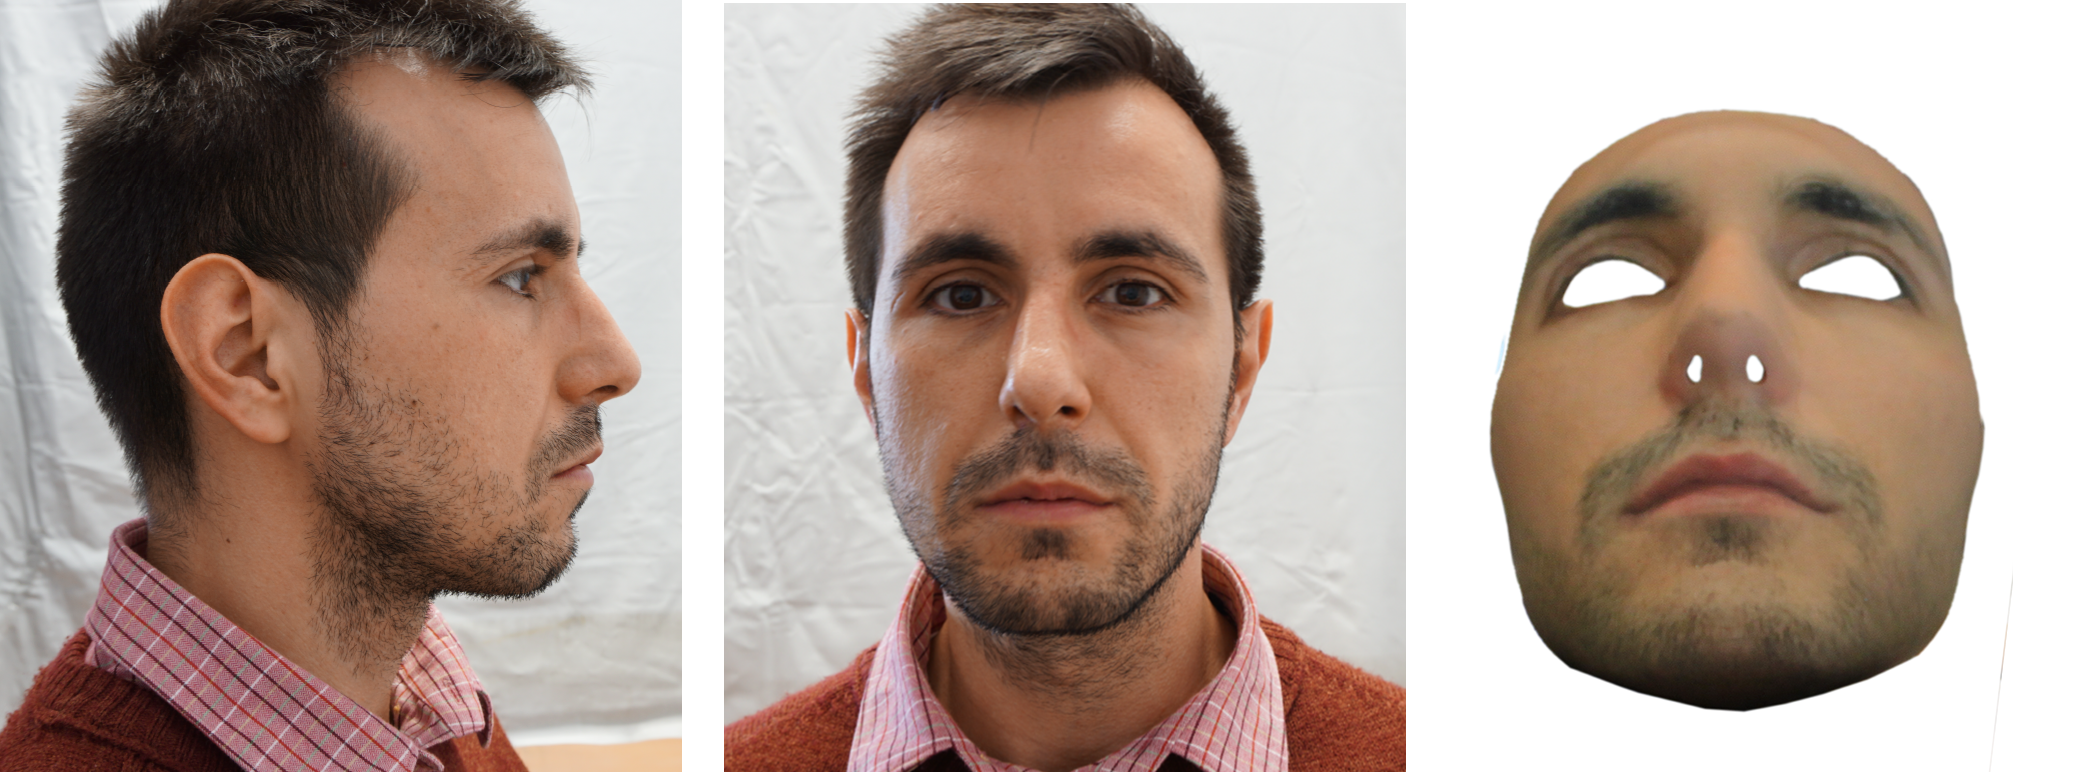
\includegraphics[width=1\linewidth]{ch-sistemasABC/images/ch-BBDDs/CONSTRUCCION_MASCARAS_3D.png}
    \caption{Máscara $3$D impresa a partir de un modelo creado por fotometría.}
    \label{fig:ConstrucionMascara3D}
\end{figure}

Además de capturas \gls{bona-fide}, se simularon ataques de presentación con $5$ tipos de \GLS{PAI} con la identidad de cada sujeto: fotografía, mascara de cartón, mascara de cartón con ojos recortados o \textit{eyeless}, pantalla y máscara $3$D (ver Fig. \ref{fig:DISTINTOS_ATAQUES_EN_FRAV_ATTACK}). A continuación se explica en que consisten los ataques con cada uno de estos \GLS{PAI}:

\medskip
\textbf{PAI fotografía} 

Consiste en presentar al sensor una fotografía impresa con la imagen del sujeto a suplantar.Se trata de una ataque simple pero muy efectivo en sistemas que no cuentan con ningún tipo de \GLS{PAD}

\medskip
\textbf{PAI máscara cartón} 

Consiste colocarse una máscara de cartón que reproduce la cara del sujeto a suplantar. A diferencia del ataque con fotografía al generar un volumen alrededor de la cara, resulta un ataque menos detectable que una fotografía plana, para sistemas \GLS{PAD} basados en profundidad.
    
\medskip
\textbf{PAI máscara cartón \textit{eyeless}}

Consiste también en llevar una máscara de cartón con la cara del sujeto a suplantar, pero en este caso los ojos de la máscara se recortan para engañar a \gls{liveness detection} \GLS{PAD} basados en la de detección de parpadeo (ver apartado \ref{sec:TiposPAD}).

\medskip
\textbf{PAI vídeo}

Consiste presentar ante el sensor la pantalla de un dispositivo electrónico que reproduce un vídeo del sujeto a suplantar. Este tipo \GLS{PAI} es también capaz de engañar a métodos \gls{liveness detection} \GLS{PAD} (ver apartado \ref{sec:TiposPAD}).

\medskip
\textbf{PAI máscara 3D}

Consiste en colocarse una máscara rígida del sujeto a suplantar.Las máscaras empleadas en \textit{\Gls{FRAV-Attack}} fueron fabricadas por la empresa \textit{ThatsMyFaces} \cite{ThatsMyFaceOnline}, mediante la impresión $3$D de un modelo estimado por fotogrametría con las vistas frontal y lateral del sujeto (ver Fig. \ref{fig:ConstrucionMascara3D}). Si bien este tipo de máscaras resultan cada día más asequibles, en \Gls{FRAV-Attack} sólo se incluyeron ataques con $10$ máscaras de este tipo. debido al coste que supondría la impresión de mascaras para los $185$ sujetos. Este tipo de máscaras es uno de los más peligrosos  ya que consiguen engañar a sistemas automáticos muy sofisticados que usan cámaras de profundidad o escáneres $3$D \cite{erdogmus2014spoofing}, \cite{jia2019survey} \cite{li2016generalized}.
\medskip

%%%%%%%%% SENSORES  %%%%%%%%%%%%
\subsection{Dispositivos de captura}\label{subsec:Dispositivos-FRAV-Attack}

\begin{figure}[t!]
\centering
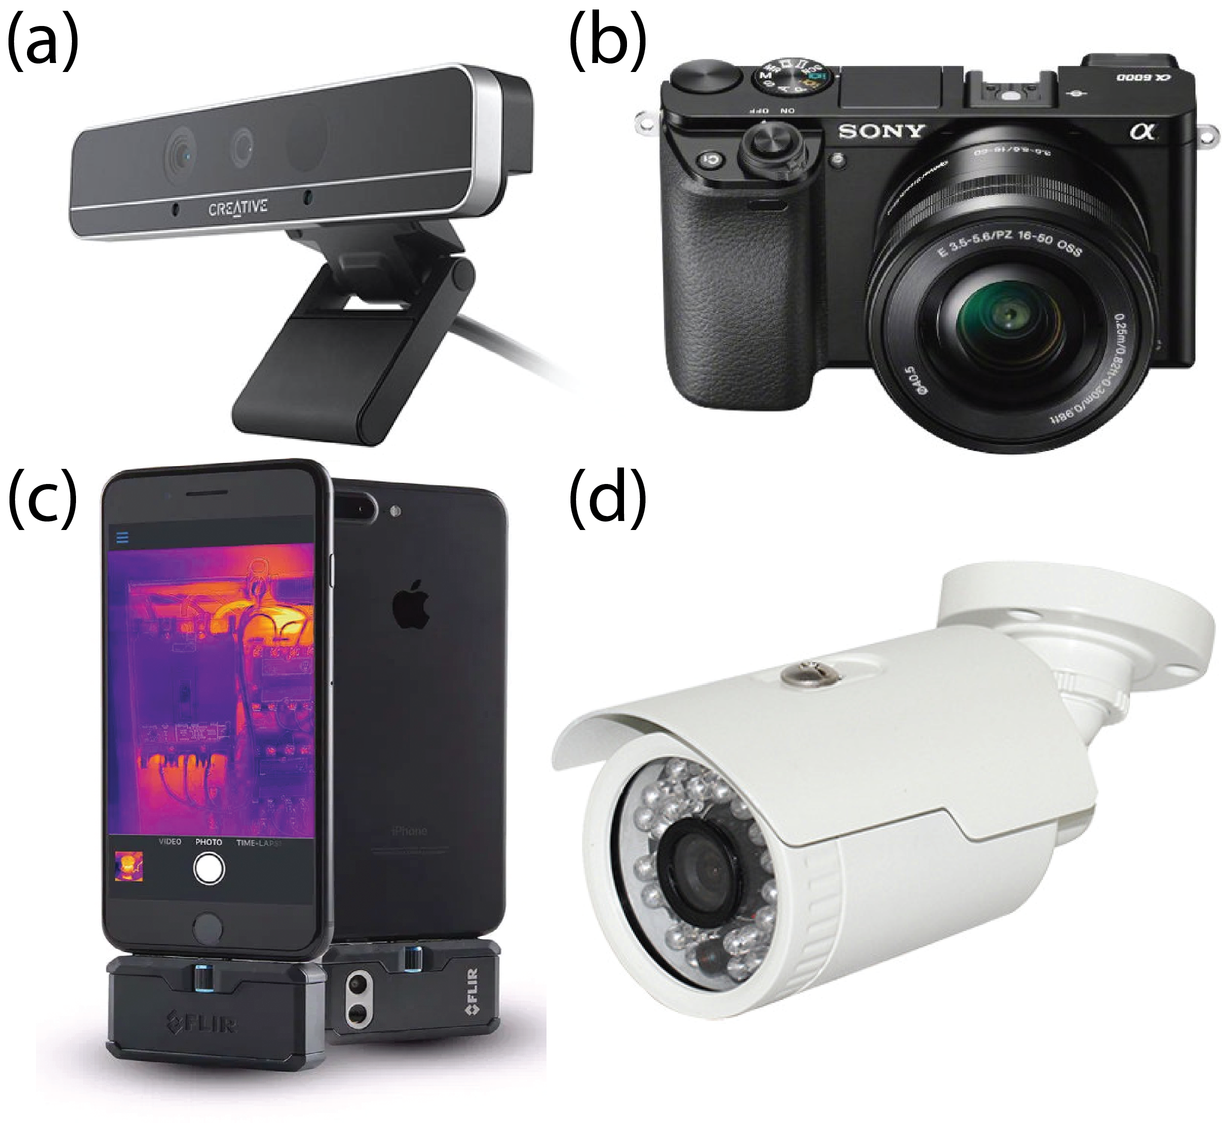
\includegraphics[width=0.6\textwidth]{ch-sistemasABC/images/ch-BBDDs/SENSORES.png}
    \caption{Dispositivos de captura de la base de datos \textit{\Gls{FRAV-Attack}}: (a) \textit{Intel\textsuperscript{\textregistered}RealSense\textsuperscript{\texttrademark}}. (b) \textit{Sony\textsuperscript{\textregistered}$\alpha6000$}. (c) \textit{\GLS{FLIR}-One} y (d) \textit{SurveillanceCam}}
    \label{fig:SENSORES}
\end{figure}

Para las capturas tanto de los \gls{bona-fide} como de los ataques de \Gls{FRAV-Attack}, se emplearon cuatro dispositivos, algunos de ellos con varios sensores que permiten capturas en rangos del espectro, diferentes al visible: \textit{Intel\textsuperscript{\textregistered}RealSense\textsuperscript{\texttrademark}}, \textit{Sony\textsuperscript{\textregistered}$\alpha6000$}, \textit{SurveillanceCam} y \textit{\GLS{FLIR}-One} (ver Fig.\ref{fig:SENSORES}). A continuación se especifican las características de cada uno de los sensores y de las capturas realizadas con ellos. 

%REALSENSE
\medskip
\textbf{Intel\textsuperscript{\textregistered}RealSense\textsuperscript{\texttrademark}}:

La cámara RealSense F$200$ \cite{RealSenseOnline} dispone de sensor \GLS{RGB} y también de un sensor \GLS{IR} que permite obtener información de profundidad ($2.5$D) mediante la lectura un un patrón de luz estructurada emitida por un proyector infrarrojo.

En \\Gls{FRAV-Attack}, con esta cámara, se grabaron vídeos de 400 fotogramas, uno con el \gls{bona-fide} y $5$ con los \GLS{PAI} correspondientes de cada sujeto. De cada fotograma se extrajeron: la imagen \GLS{RGB} con una resolución de $1920\times1080$, la imagen \GLS{IR} con una resolución de $640\times480$ y la matriz de profundidades, también con $640\times480$ de resolución. (aproximadamente $1$ millón imágenes en total). En Fig. \Ref{fig:USUARIOS_RELASENSE} se pueden ver las segmentación facial de tres sujetos de \Gls{FRAV-Attack}, en cada una de estas imágenes.

%SONY
\medskip
\textbf{Sony\textsuperscript{\textregistered}$\mathbf{\alpha6000}$}

Cámara fotográfica con un sensor \GLS{RGB} de alta resolución capaz de capturar imágenes de $24.3$ MP y vídeos ($4$HD) a $1080$. 

Para \Gls{FRAV-Attack} con este dispositivo se capturaron, de cada sujeto, tres imágenes \gls{bona-fide} de $6000\times4000$ píxeles con pose frontal, perfil derecho y perfil izquierdo. Y una imagen también de $6000\times4000$ píxeles de cada uno de los \GLS{PAI} (aproximadamente $1500$ imágenes). 

Gracias a la calidad de las imágenes obtenidas con este sensor se han utilizado para la construcción de los diferentes \GLS{PAI} (ver Fig. \ref{fig:ConstrucionMascara3D}). 

%FLIR TERMICO
\medskip
\textbf{\gls{FLIR}-One} 

La cámara \gls{FLIR}-One \cite{FLIROnline} tiene de un sensor \GLS{RGB} y otro térmico capaz de capturar la temperatura emitida por los objetos en el de infrarrojo medio con un rango de temperaturas entre -$4^{\circ}$F to $248^{\circ}$F (-$20^{\circ}$C to $120^{\circ}$ C). 

En \Gls{FRAV-Attack} se tomaron tres capturas con el \gls{bona-fide} de cada sujeto en pose frontal, perfil derecho y perfil izquierdo, y una captura de los \GLS{PAI} correspondientes. Cada captura de este dispositivo genera dos matrices de $160\times120$ con la información térmica: \textit{ThermalLinearFlux} y \textit{ThermalRadiometricKelvin}, y dos imágenes \GLS{RGB} de $640\times480$ píxeles: \textit{VisualJPEGImage}, en formato \GLS{JPEG} y \textit{VisualYCbCr888Image}, en formato \Gls{YCbCr} (aproximadamente $6000$ imágenes).  

A las imágenes generadas se les puede aplicar paletas de color atendiendo a las matrices de temperatura para analizar determinadas propiedades térmicas: \textit{Arctic}, \textit{Coldest}, \textit{Hottest}, \textit{Contrast}, \textit{Gray}, \textit{Iron}, \textit{Lava}, \textit{Rainbow}, \textit{Whell} (ver Fig.\ref{fig:DISTINTAS_PALETAS_TERMICAS} y Fig. \ref{fig:DISTINTOS_ATAQUES_DISTINTAS_PALETAS}).

%INFRARROJO
\medskip
\textbf{Surveillance-Cam}

% \begin{figure}[t!]
% \centering
% 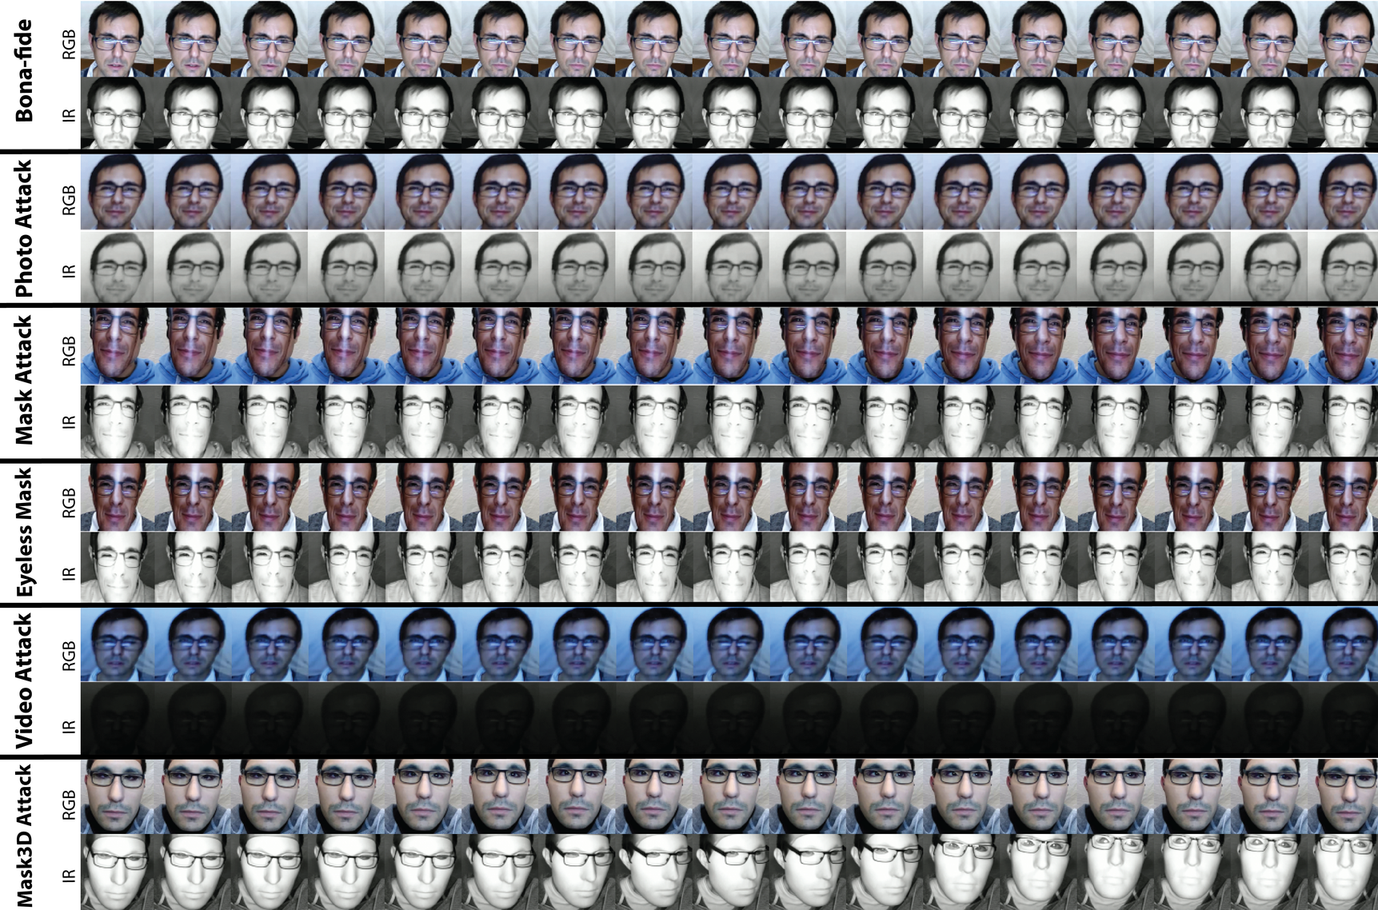
\includegraphics[width=1\textwidth]{ch-sistemasABC/images/ch-BBDDs/MUESTRAS_IR.png}
%     \caption{Fotogramas de los vídeos de \textit{\Gls{FRAV-Attack}} con el cámara \textit{SurveillanceCam}.}
%     \label{fig:MUESTRAS_IR}
% \end{figure}

El dispositivo \textit{Surveillance-Cam} es una cámara de alta resolución, empleada en labores de vídeo-vigilancia, capaz de capturar imágenes y vídeos, en\GLS{RGB} y en \GLS{IR}. Además dispone de un sistema integrado de iluminación infrarroja.

En \Gls{FRAV-Attack} de cada sujeto se grabaron vídeos de $400$ fotogramas, uno con el \gls{bona-fide} y 5 con los \GLS{PAI} correspondientes. De cada fotograma se extrajeron: la imagen \GLS{RGB} y la \GLS{IR}, ambas con una resolución $1920\times1080$ píxeles. (casi un 1 millón imágenes en total). En Fig. \Ref{fig:MUESTRAS_IR} se pueden ver imágenes extraídas de los vídeos de un sujeto de \Gls{FRAV-Attack}.


\begin{landscape}
\begin{figure}[t!]
\centering
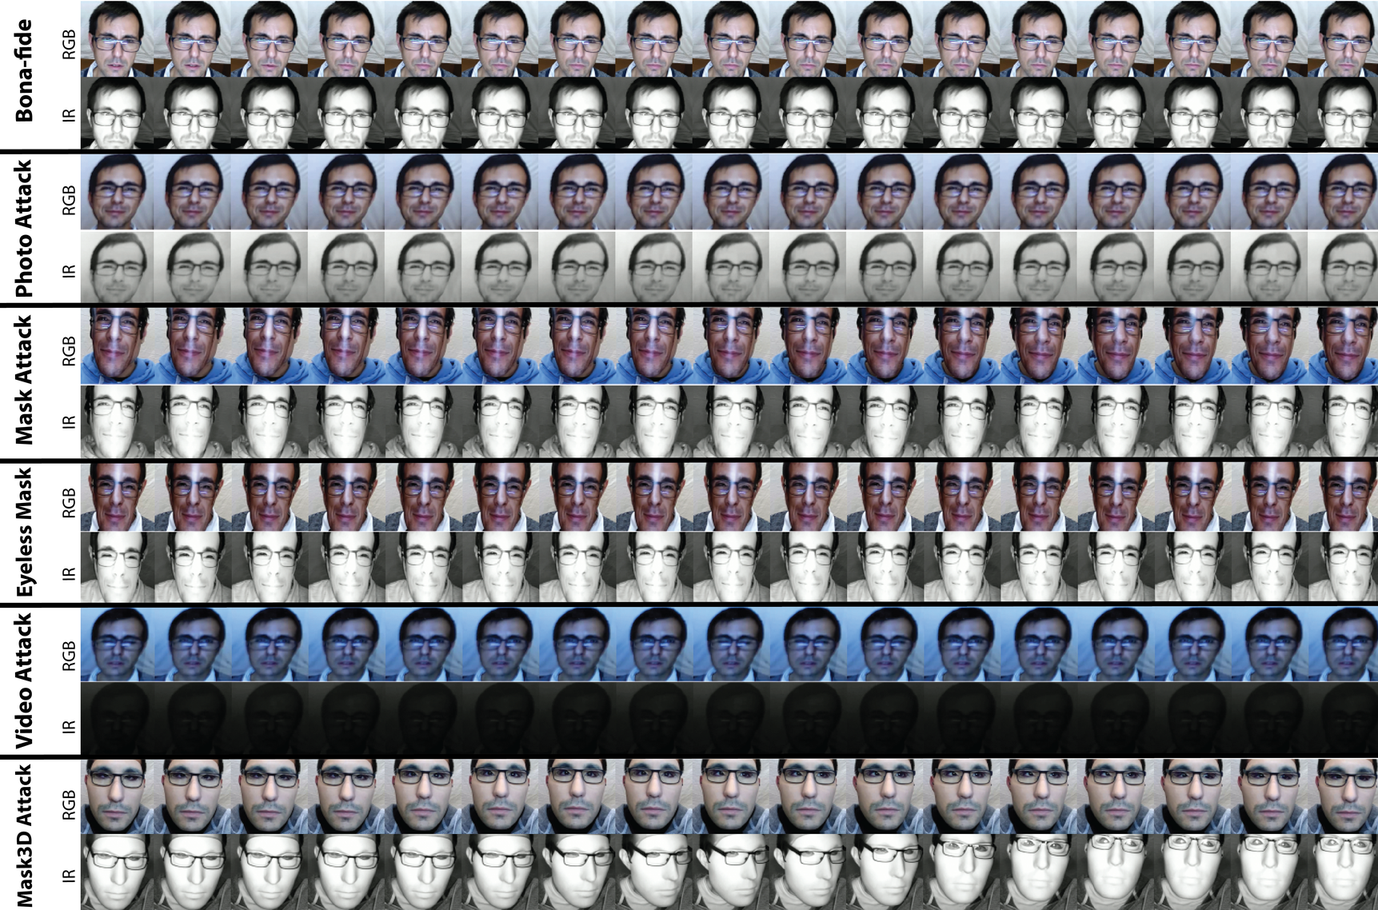
\includegraphics[width=1.4\textwidth]{ch-sistemasABC/images/ch-BBDDs/MUESTRAS_IR.png}
    \caption{Fotogramas de los vídeos de \Gls{FRAV-Attack} con el cámara \textit{SurveillanceCam}.}
    \label{fig:MUESTRAS_IR}
\end{figure}
\end{landscape}

\begin{landscape}
\begin{figure}
    \centering
    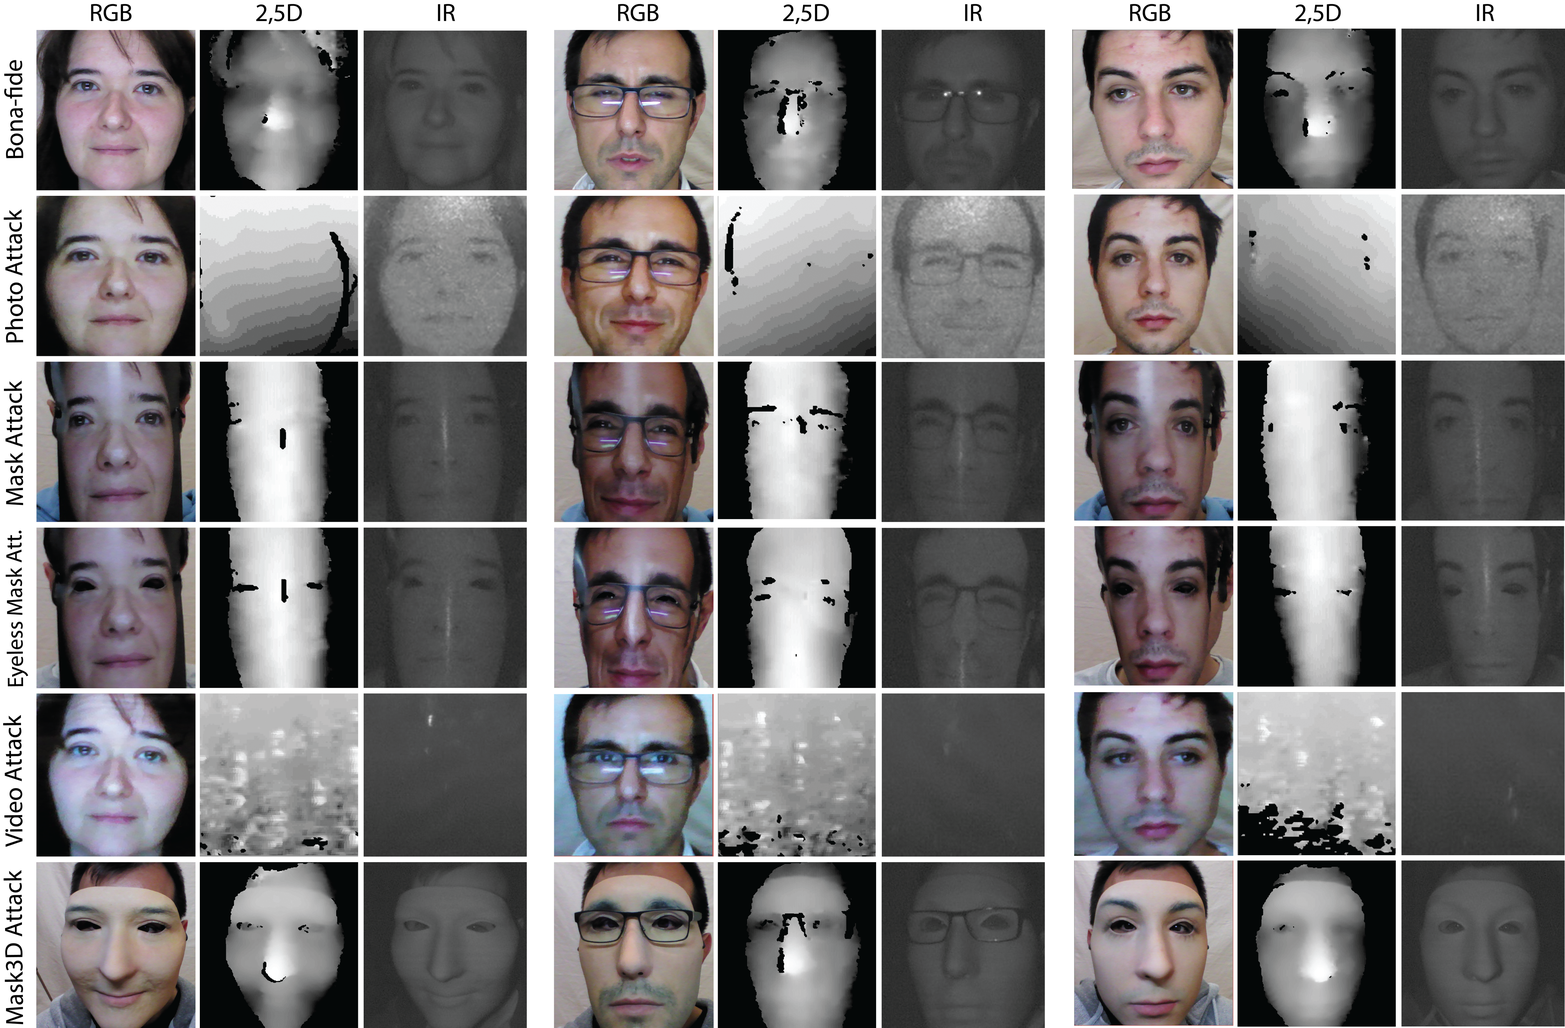
\includegraphics[width=1.4\textwidth]{ch-sistemasABC/images/ch-BBDDs/USUARIOS_REAL_SENSE.png}
    \caption{Capturas de \Gls{FRAV-Attack} con el cámara \textit{Intel-RealSemse}.}
    \label{fig:USUARIOS_RELASENSE}
\end{figure}
\end{landscape}

\begin{landscape}
 \begin{figure}
  \centering
  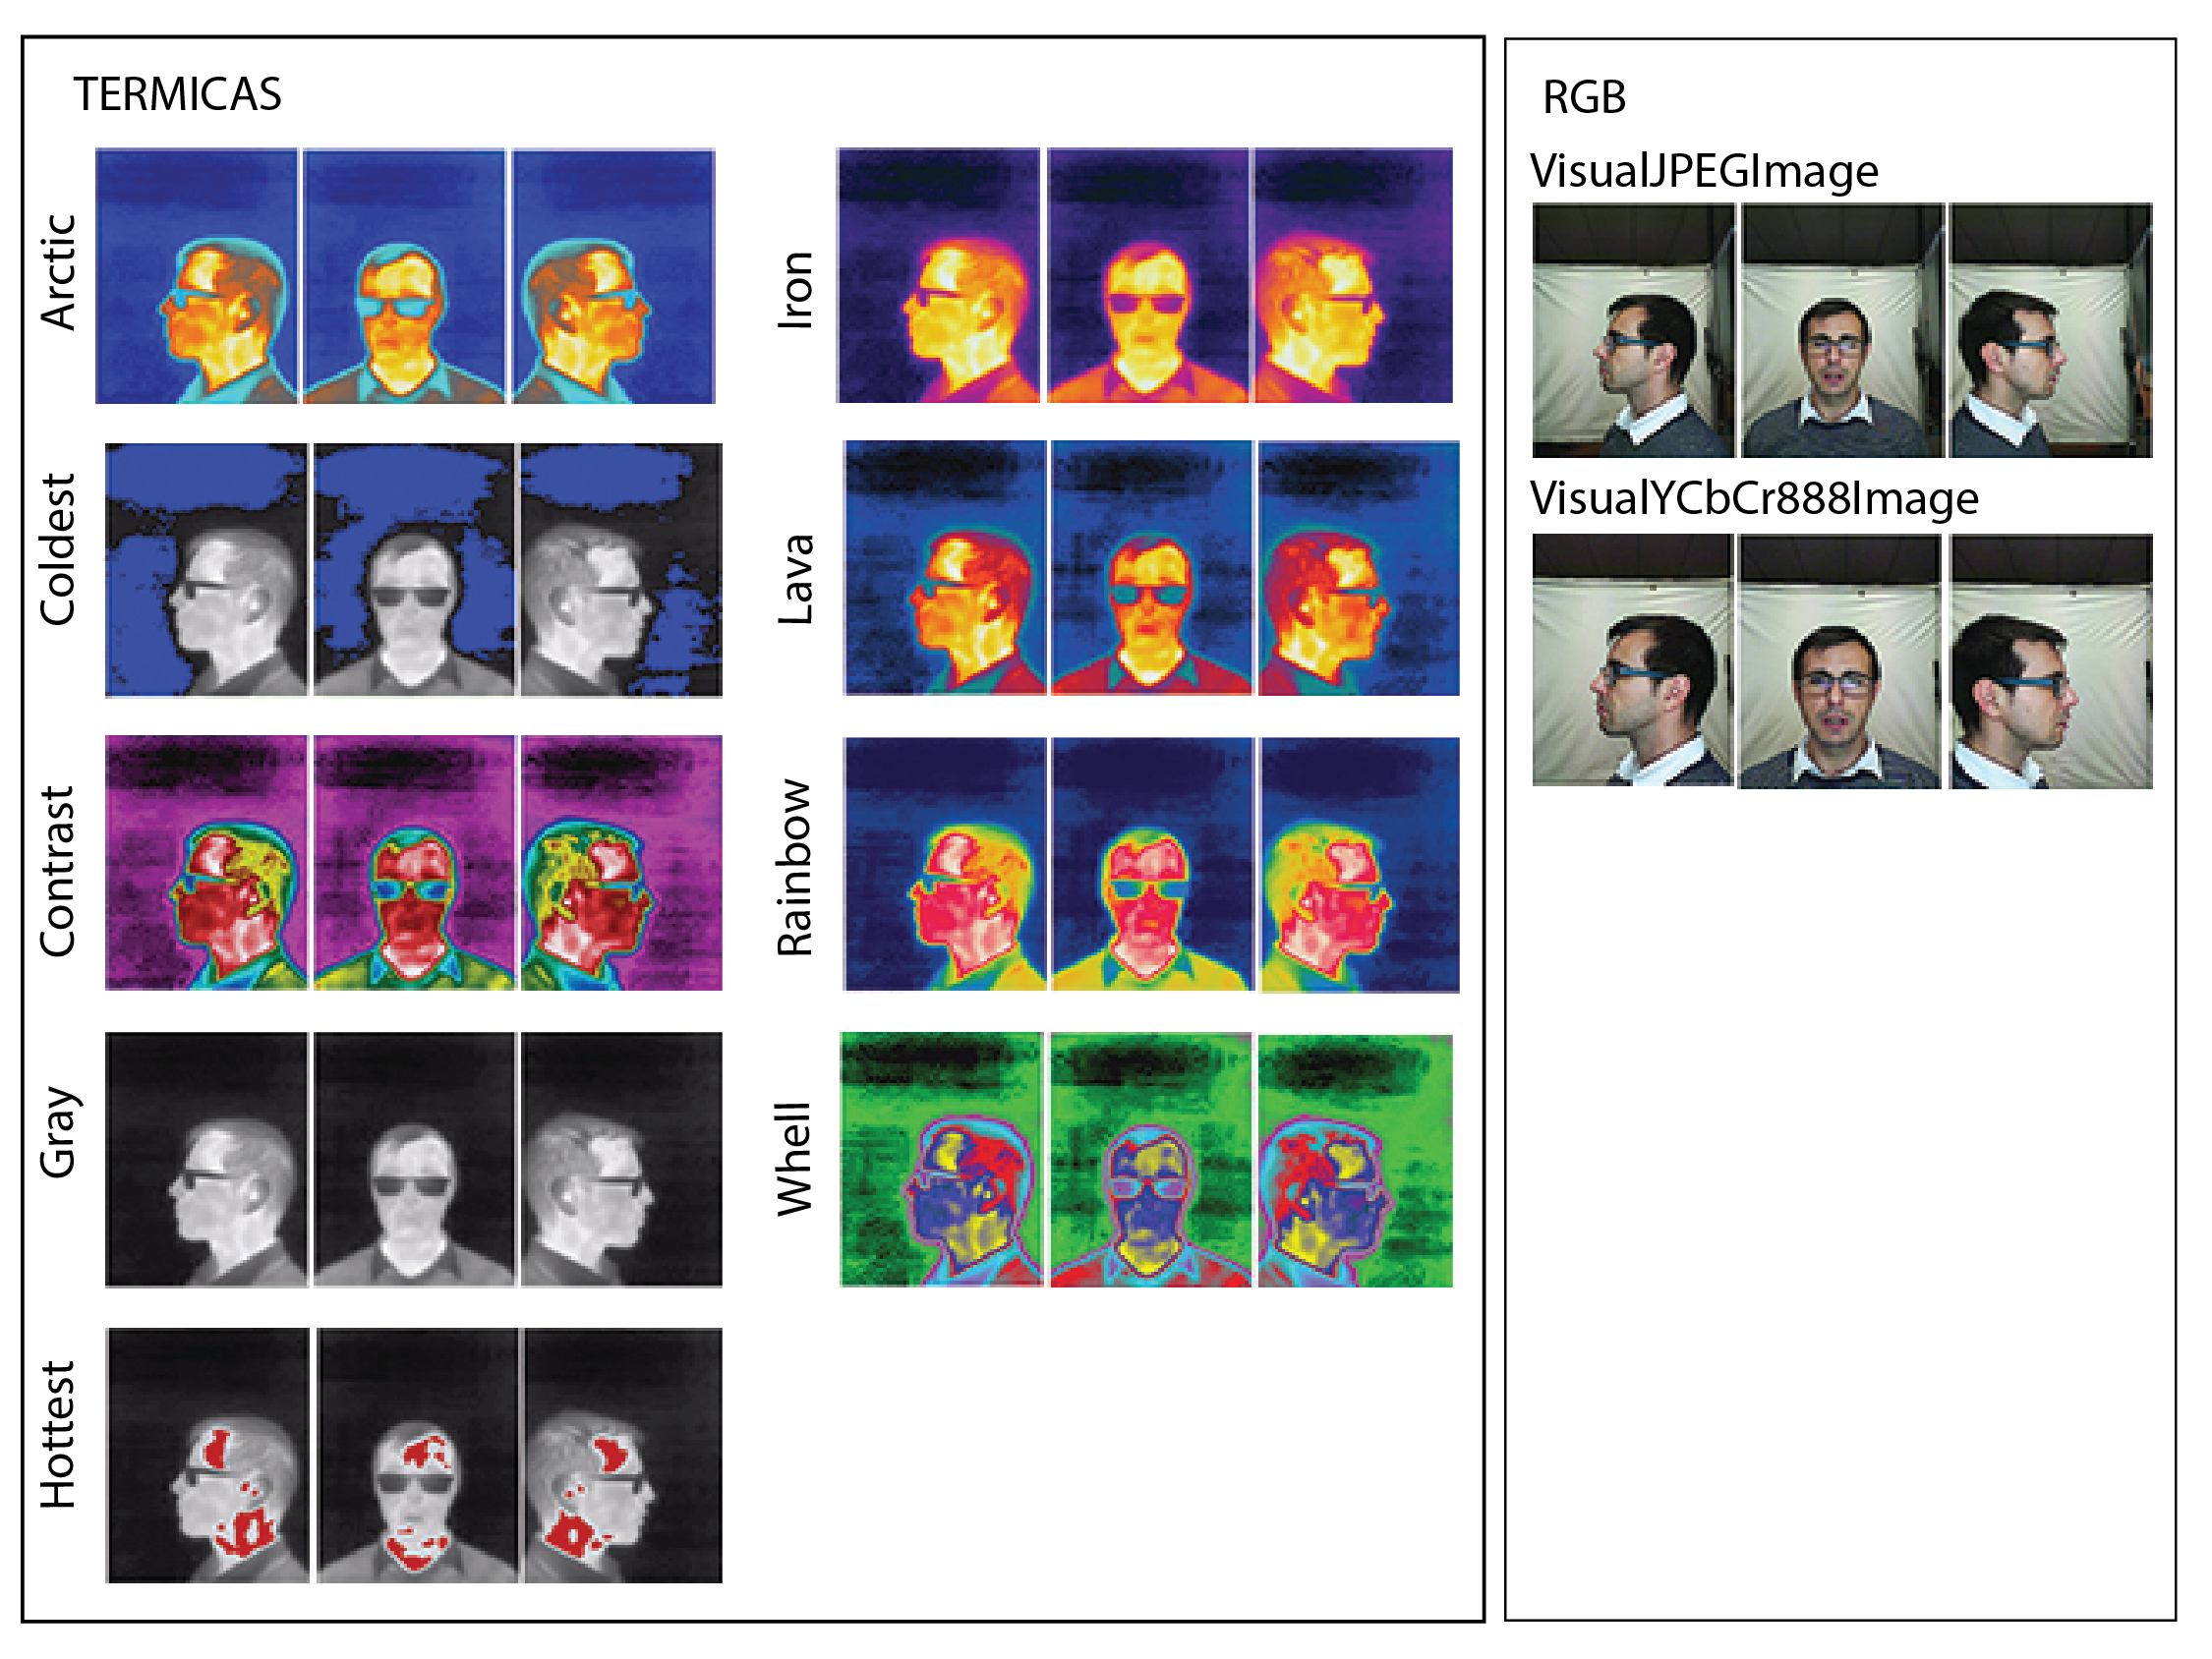
\includegraphics{ch-sistemasABC/images/ch-BBDDs/DISTINTAS_PALETAS_TERMICAS.png}
        \caption{Capturas de \Gls{FRAV-Attack} con el sensor térmico \GLS{FLIR}}
        \label{fig:DISTINTAS_PALETAS_TERMICAS}
 \end{figure}
\end{landscape}

\begin{landscape}
 \begin{figure}
  \centering
  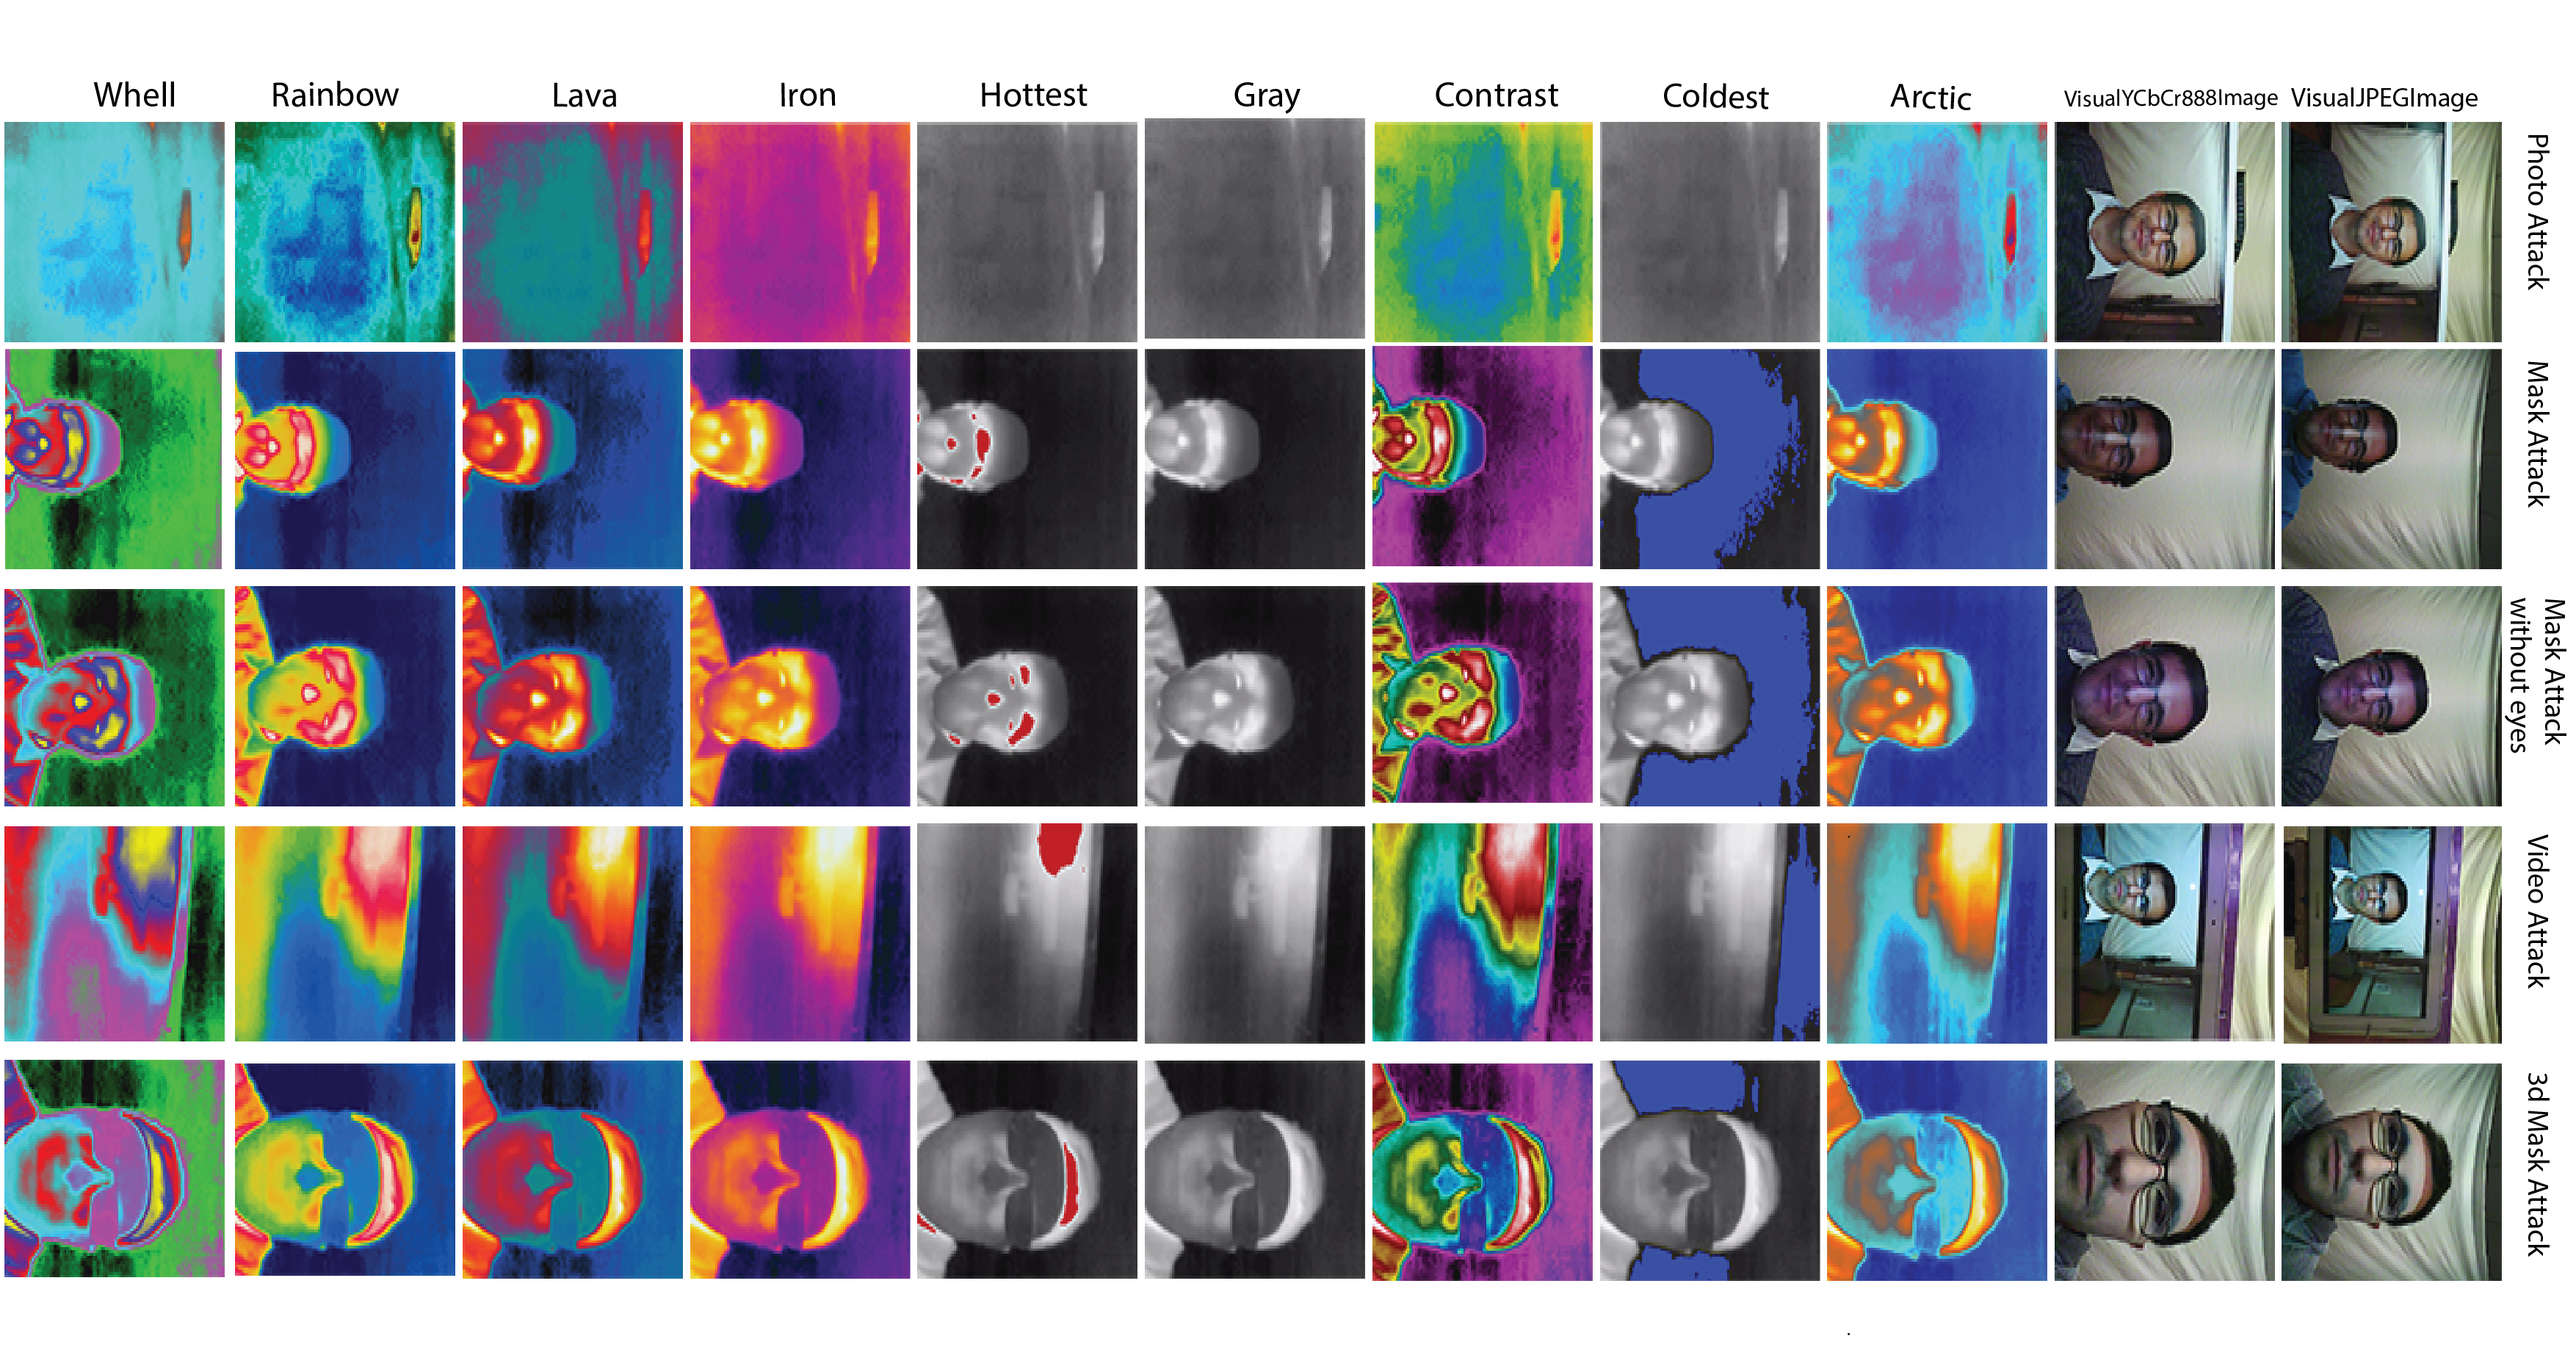
\includegraphics[width=1.5\textwidth]{ch-sistemasABC/images/ch-BBDDs/DISTINTOS_ATAQUES_DISTINTAS_PALETAS.png}
        \caption{Capturas de \Gls{FRAV-Attack} con el sensor térmico \GLS{FLIR}. Con cada uno de los ataques contemplados.}
        \label{fig:DISTINTOS_ATAQUES_DISTINTAS_PALETAS}
 \end{figure}
\end{landscape}


%%%%%%%%%%%%%%%%%%%%% BASES DE DATOS PARA SISTEMAS ABC  %%%%%%%%%%%%%%%%%%%%%%% 
\section{Bases de datos para sistemas ABC}\label{sec:BBDD-ABC}

En esta sección se presentan dos bases de datos capturadas por dispositivos \GLS{ABC} en cruces de fronteras reales. \Gls{FRAV-ABC} que incluye únicamente las imágenes que forman parte de un cruce \gls{bona-fide}: imágenes \gls{chip} e imágenes \gls{vivo bona-fide}. Sin embargo en \Gls{FRAV-ABC-Attack} considera además ataques de presentación en las imágenes \gls{vivo}. También en \Gls{FRAV-ABC-Attack} un subconjunto de los datos se capturó en un sistemas \GLS{ABC} \textit{<<Segregated Two Step>>}, lo que implica dos procesos de verificación biométrica. es decir dos capturas \gls{vivo}. En el apartado \ref{subsec:FRAV-ABC-ATTACK-DOS_PASOS} se explica el formato y las características de este subconjunto de datos.

El acceso a cruces de fronteras reales está muy controlado y limitado por razones de seguridad. La posibilidad de capturar los datos descritos en esta sección fue gracias la participación del grupo de investigación \GLS{FRAV} de la universidad \GLS{URJC} en el proyecto europeo FP$7$ \GLS{ABC4EU}, donde colaboró en la implantación de prototipos de sistemas \GLS{ABC} en fronteras aeroportuarias, fronteras terrestres y fronteras marítimas.

Se realizó una experiencia piloto en el Adolfo Aeropuerto Suárez Madrid-Barajas T$4$-S internacional terminal de llegadas en diciembre de $2016$. Este aeropuerto, que sirve a la capital de España y al centro de la Península Ibérica, es el aeropuerto más concurrido de España, y el quinto en Europa y el $24$º en el mundo en cuanto al tráfico de viajeros. En $2015$ alcanzó un de casi $47$ millones de viajeros \cite{ACI2016}.

%%%%%%%%%%%%%%%%%%%%% FRAV ABC  %%%%%%%%%%%%%%%%%%%%%%% 
\subsection{FRAV-ABC}\label{subsec:FRAV-ABC}

% \Figure[ht]()[width=.9\linewidth]{images/FRAV-ABC-Images.png}
%  {Examples of \textit{FRAV-ABC} data set images. Passport \textit{chip} images (top) and snap-shot images taken in the border scenario (bottom).\label{fig:SAMPLES-FRAV-ABC1}}

\begin{figure}[ht]
     \centering
     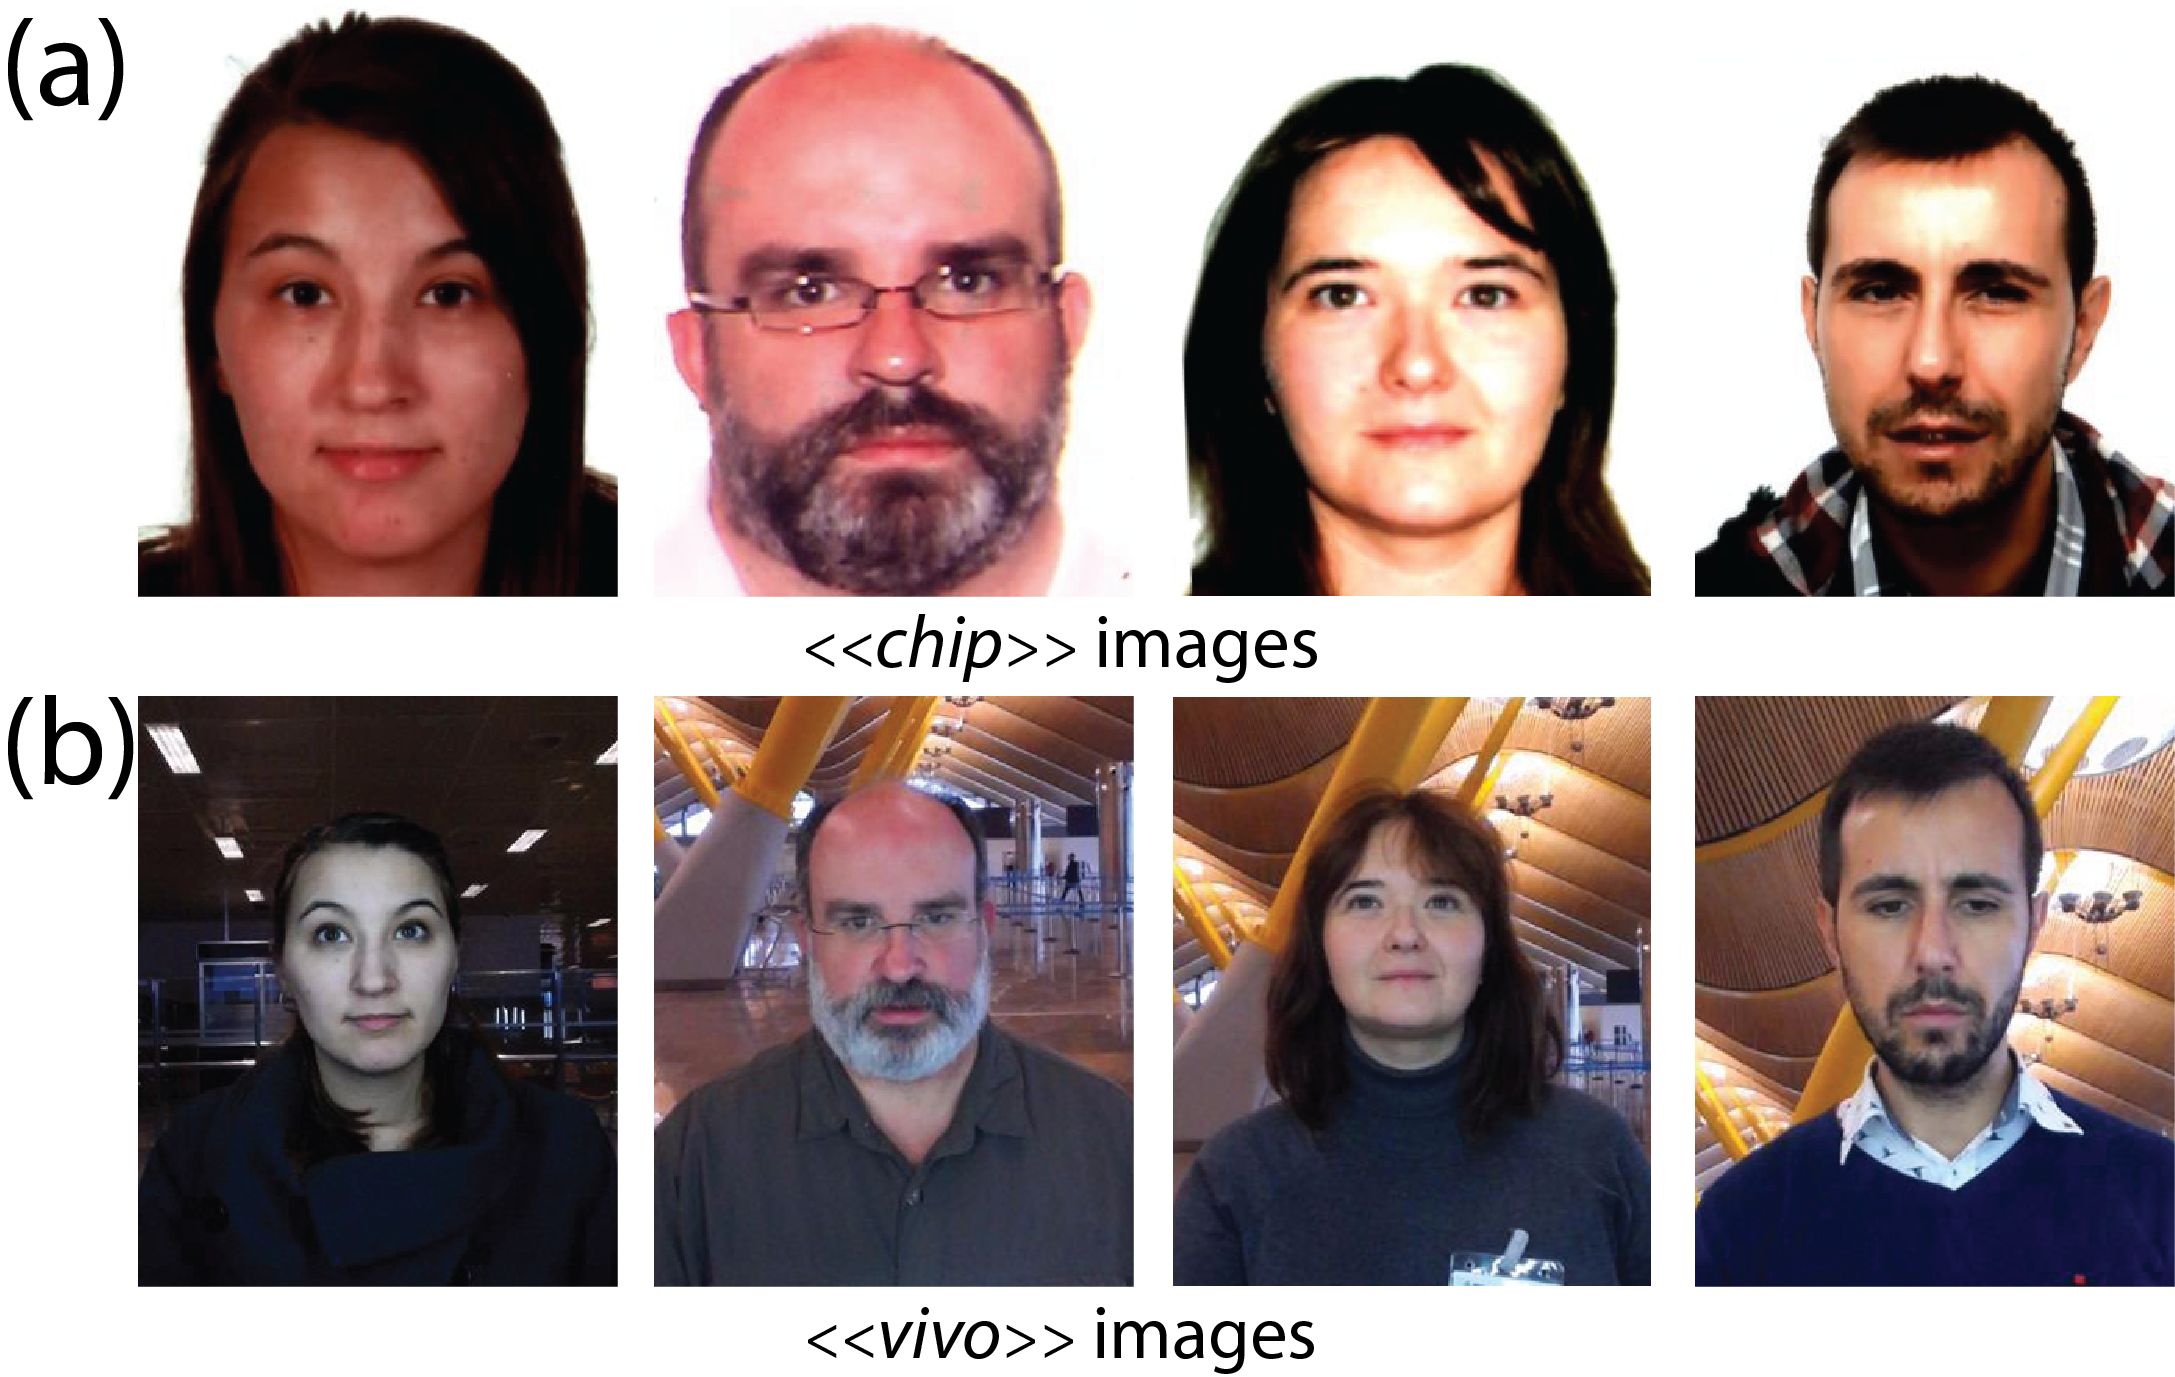
\includegraphics[width=0.8\textwidth]{ch-sistemasABC/images/ch-BBDDs/CHIP_VIVO_IMAGENES.png}
     \caption{Imágenes de sujetos de la base de datos \textit{\Gls{FRAV-ABC}}. (a) Imágenes del \gls{chip} del \gls{e-passport} y (b) Imágenes \gls{vivo} adquiridas por un sistema \GLS{ABC} en un cruce de fronteras real.}
     \label{fig:SAMPLES-FRAV-ABC1}
\end{figure}

En este apartado se describe la base de datos \Gls{FRAV-ABC}\footnote{La base de datos \Gls{FRAV-ABC} fue diseñada y recopilada por el grupo de investigación \GLS{FRAV} de la \GLS{URJC}\cite{urjcOnline} gracias a la colaboración de este grupo en el proyecto \GLS{ABC4EU}\cite{ABC4EUOnline} durante la implantación de sistemas \GLS{ABC} pilotos, en la terminal T$4$ en el Aeropuerto Alfonso Suarez Madrid-Barajas y en el puerto marítimo de Algeciras.}, compuesta por 1185 sujetos, 640 mujeres y 530 hombres, con un rango de edades entre 18 y 74 años. El $70$\% oscilaba entre $25$ y $50$ años de edad. De cada sujeto se dispone de dos imágenes: Una imagen con características similares a las almacenadas en los \gls{eMRTD} conocida como \gls{chip} y una imagen capturada en un dispositivo \GLS{ABC} en un cruce de fronteras real, conocida como \gls{vivo} (ver Fig. \ref{fig:SAMPLES-FRAV-ABC1}). En suma. 1185 imágenes \gls{chip} y 1185 imágenes \gls{vivo}.

\medskip
\textbf{\gls{chip}}

Las imágenes \gls{chip} son imágenes \textit{RGB} con una resolución de $250\times300$ píxeles que cumplen la normativa estándar de \GLS{ICAO} Doc $9303$ \cite{doc20069303} para \gls{eMRTD}.

\medskip
\textbf{\gls{vivo}}

Las imágenes \gls{vivo} son imágenes \GLS{RGB} con una resolución de $300\times300$ píxeles, capturadas \textit{in situ} en un cruce de fronteras real por un dispositivo \GLS{ABC} operativo.
\medskip
   
%%%%%%%%%%%%%%%%%%%%% FRAV ABC ATTACK  %%%%%%%%%%%%%%%%%%%%%%% 
\subsection{FRAV-ABC-Attack: Ataques de presentación en sistemas ABC}\label{subsec:FRAV-ABC-ATTACK}

\begin{figure}[ht]
    \centering
    \includegraphics[width=1\linewidth]{ch-sistemasABC/images/ch-BBDDs/SAMPLES_DE_FRAV_ABC.png}
    \caption{Muestras de la base de datos \Gls{FRAV-ABC-Attack}: (a) <<chip>>. (b) \gls{vivo bona-fide}. (c) \gls{vivo ataque} máscara $3$D. (d) \gls{vivo ataque} Fotografía. (e) \gls{vivo ataque} máscara catón. (f) \gls{vivo ataque} vídeo. (g) \gls{vivo ataque} camiseta.}
    \label{fig:SAMPLES-FRAV-ABC-ATTACK}
\end{figure}

\begin{figure}[ht]
    \centering
    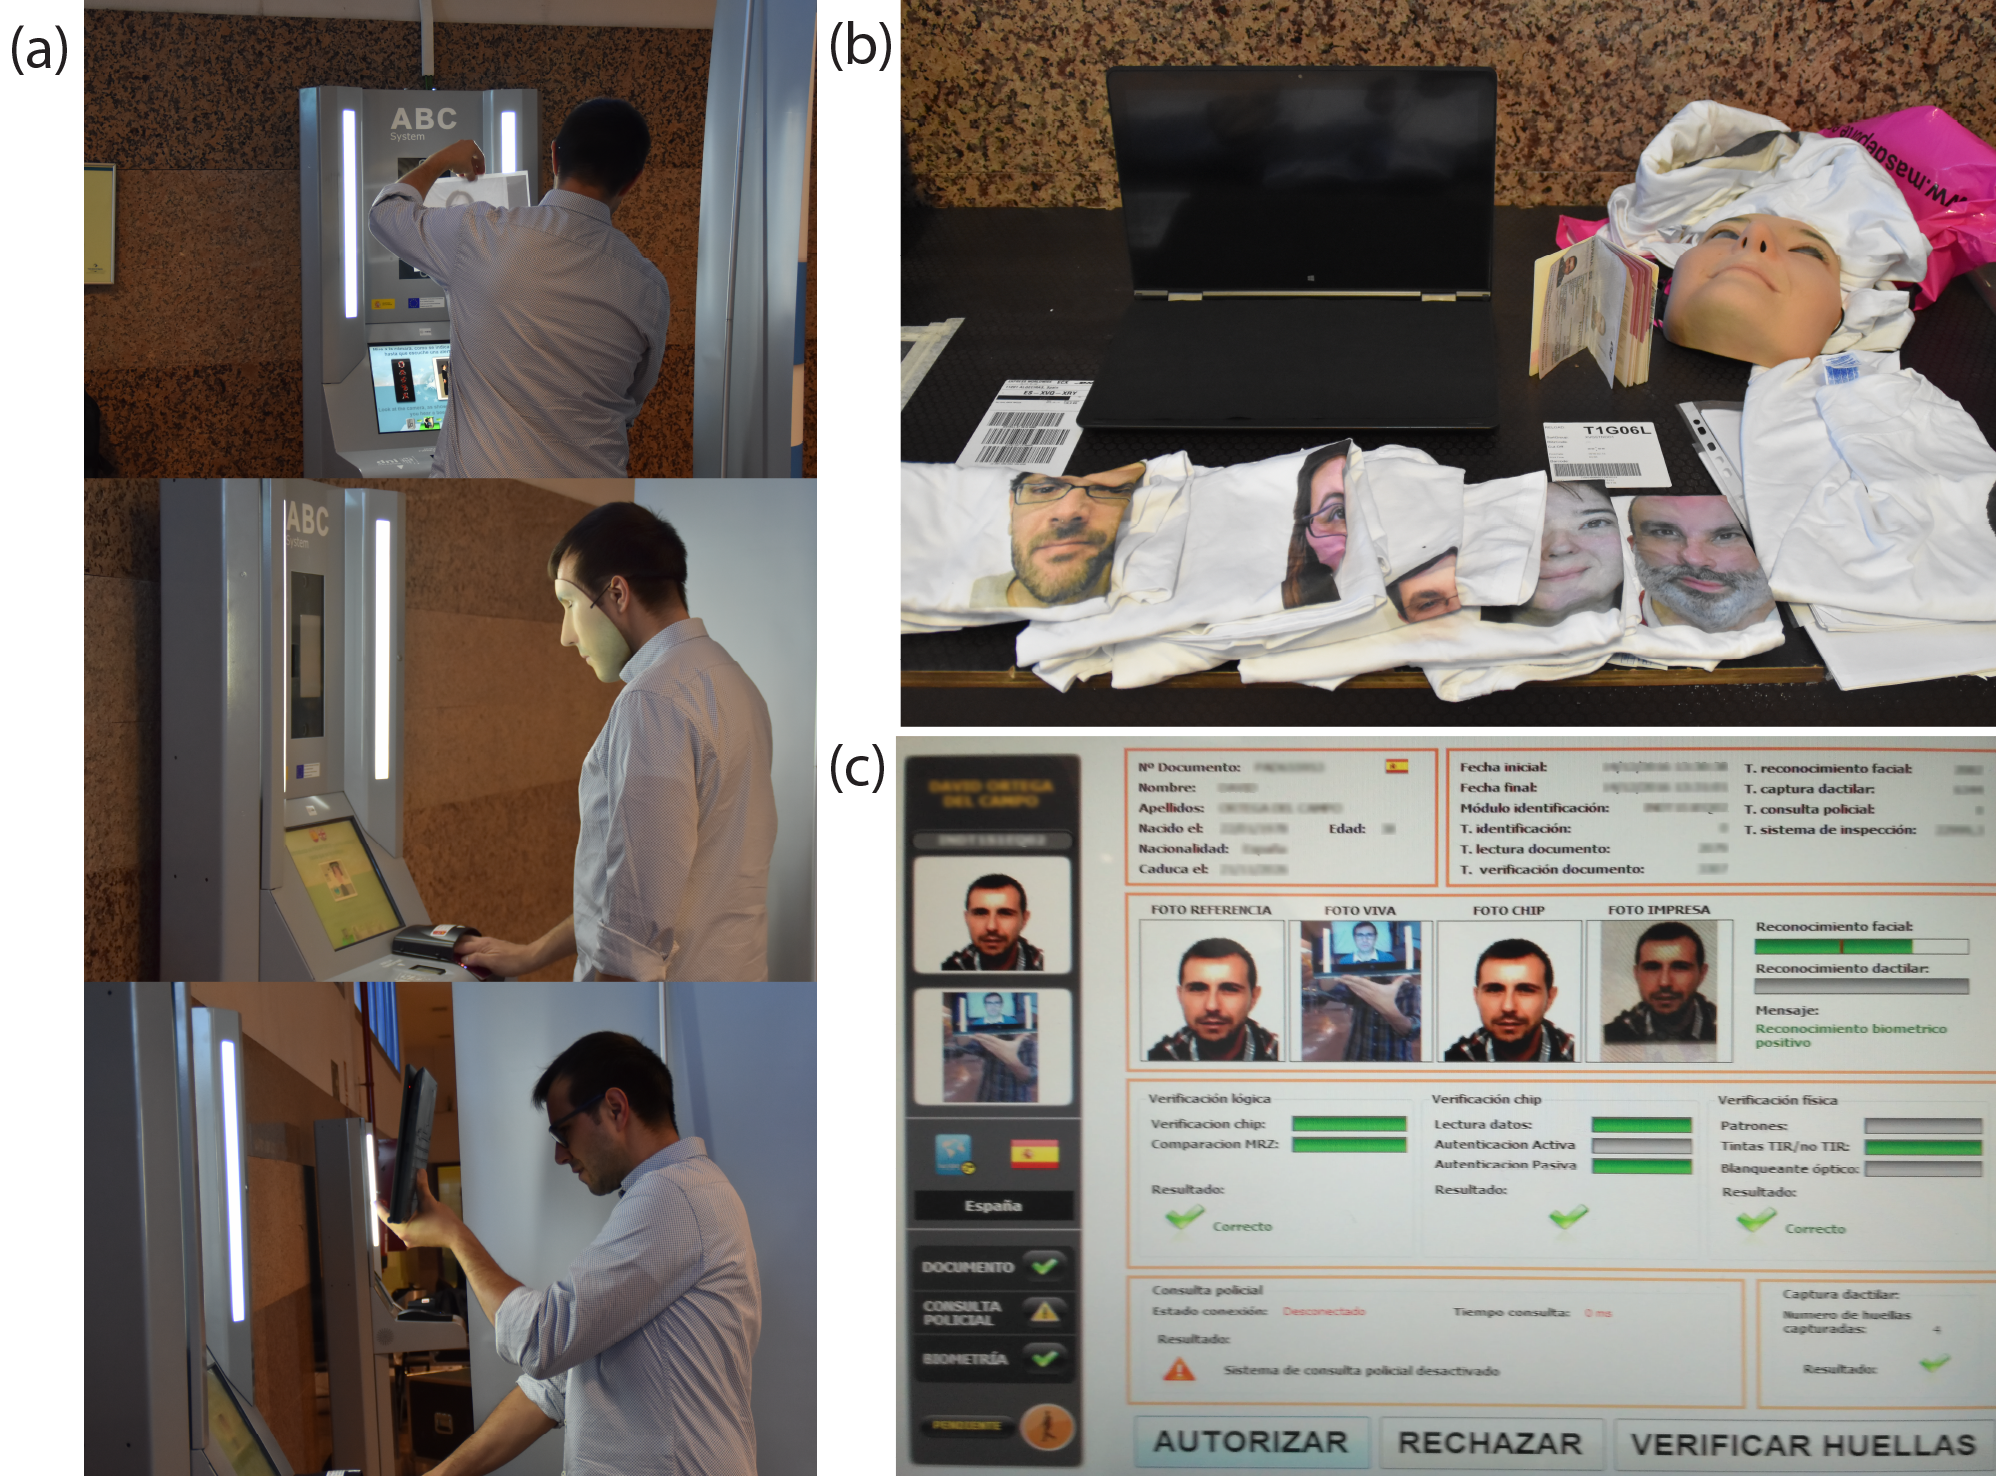
\includegraphics[width=1\linewidth]{ch-sistemasABC/images/ch-BBDDs/CAPTURA_FRAV_ABC.png}
    \caption{Imágenes de la adquisición de la base de datos \Gls{FRAV-ABC}: (a) Presentación de ataques en el dispositivo. (b) \Glspl{PAI} de los distintos ataques. (c) Pantalla de traza de los dispositivos.}
    \label{fig:AdquisicionFRAVABC}
\end{figure}

En esta sección se describe la base de datos \gls{FRAV-ABC-Attack}\footnote{La base de datos \Gls{FRAV-ABC-Attack} se capturó en las mismas circunstancias que \Gls{FRAV-ABC}.}, compuesta por 300 sujetos (160 mujeres y 140 hombres), ya incluidos \gls{FRAV-ABC} y cuyos datos fueron capturados también un dispositivo \GLS{ABC} en un cruce de fronteras real (ver Fig. \ref{fig:AdquisicionFRAVABC}). Pero, en este caso se incluyeron: la imagen \gls{chip} y varias \gls{vivo}: un  \gls{vivo bona-fide} y 5 \gls{vivo ataque}. Las imágenes \gls{chip} con formato \GLS{RGB} de $300\times300$ píxeles y todas las imágenes \gls{vivo}, también \GLS{RGB} de $300\times300$ píxeles. En suma, 300 imágenes \gls{chip}, 300 \gls{vivo bona-fide} y 1500 \gls{vivo ataque}.

\medskip
\textbf{\textit{<<vivo bona-fide>>}}

Las imágenes \gls{vivo bona-fide} son imágenes capturadas \textit{in situ} en un cruce de fronteras real por un dispositivo \GLS{ABC} operativo con una presentación del sujeto genuino.

\medskip
\textbf{\textit{<<vivo ataque>>}}

Las imágenes \gls{vivo ataque} son imágenes capturadas \textit{in situ} en un cruce de fronteras real por un dispositivo \GLS{ABC} operativo, con presentaciones con algún \GLS{PAI} de los contemplados: Máscara $3$D, fotografía, máscara de cartón, vídeo y camiseta (Ver Fig. \ref{fig:SAMPLES-FRAV-ABC-ATTACK}).
\medskip

Los ataques contemplados para la realización de esta base de datos son similares a los que se incluyen en \Gls{FRAV-Attack} (ver Sección \ref{subsec:FRAV-ABC-ATTACK}) pero además se ha añadido un nuevo \GLS{PAI}, el ataque con camiseta, que consiste en llevar una prenda de vestir con la fotografía serigrafiada del viajero genuino, este \GLS{PAI} permite engañar al sistema si la detección facial encuentra la cara estampada antes que la del impostor (ver Fig. \ref{fig:SAMPLES-FRAV-ABC-ATTACK} (g)).

%%%%%%%%%%%%%%%%%%%%% FRAV ABC ATTACK DOS PASOS SEGREGADOS %%%%%%%%%%%%%%%%%%%%%%% 
\subsection{FRAV-ABC-Attack \textit{<<Segregated Two Step>>}}\label{subsec:FRAV-ABC-ATTACK-DOS_PASOS}

\begin{figure}[ht]
     \centering
     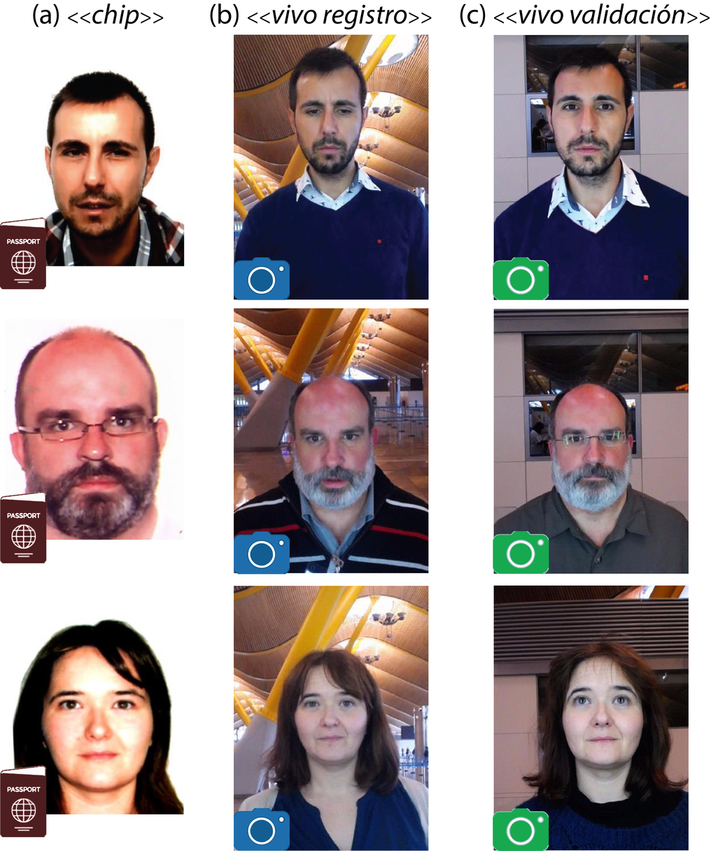
\includegraphics[width=0.6\textwidth]{ch-sistemasABC/images/ch-BBDDs/VERIFICACION_DAVID_ENRIQUE_CRISITNA_DOS_PASOS.png}
     \caption{Imágenes \gls{FRAV-ABC-Attack} en un sistema \GLS{ABC} \textit{<<Segregated Two Step>>} con doble verificación: (a) Imagen \gls{chip}. (b) Imagen \gls{vivo registro} en \GLS{RTP}  y (c) Imagen \gls{vivo validacion} en \GLS{EES}.}
     \label{fig:Imagenes_ABC_Attack_dosPasos}
\end{figure}

Los datos de $100$ sujetos de la base de datos de \Gls{FRAV-ABC-Attack} se adquirieron con sistemas \GLS{ABC} \textit{<<Segregated Two Step>>} lo que implica dos capturas biométricas, una en la etapa de \GLS{RTP} y otra en \GLS{EES} (ver apartado: \ref{subsec:ArquitecturaLogicaABC}). De cada sujeto se incluyeron su imagen \gls{chip}, \gls{vivo registro} capturada en la tapa \GLS{RTP} y \gls{vivo validacion} capturada en la etapa \GLS{EES} (ver Fig. \ref{fig:Imagenes_ABC_Attack_dosPasos}).

\medskip
\textbf{\gls{vivo registro}}

Las imágenes \gls{vivo registro} son imágenes capturadas en la etapa de \GLS{RTP} \textit{in situ} por un dispositivo \gls{e-kiosk} de un cruce de fronteras real.

\medskip
\textbf{\gls{vivo validacion}}

Las imágenes \gls{vivo validacion} son imágenes capturadas en la etapa de \GLS{EES} \textit{in situ} por un dispositivo \gls{e-gate} de un cruce de fronteras real.
\medskip

En cada una de las etapas también se simularon ataques con lo que para cada etapa se obtuvieron capturas: \gls{vivo registro bona-fide}, \gls{vivo registro ataque} y \gls{vivo validacion bona-fide} y \gls{vivo validacion ataque}.

%%%%%%%%%%%%% BASESD DE ATOS PARA SISTEMAS ABC ONTHEFLY %%%%%%%%%%%%%%%%%%%% 
\section{Bases de datos para sistemas ABC \textit{OnTheFly}}\label{sec:BBDD-OnTheFly}

En estas sección se describen dos bases de datos diseñadas para sistemas \GLS{ABC} con captura dinámica: \Gls{FRAV-OnTheFly} y \Gls{FRAV-ABC-OnTheFly}. Se puede encontrar mas información sobre este tipo de sistemas en la Sección \ref{sec:tiposABC}. Todas las capturas incluidas en estas bases de datos son vídeos. En el caso de \Gls{FRAV-OnTheFly}, vídeos capturados en un laboratorio en condiciones controladas, con sujetos que simulan el comportamiento de viajeros frente a un sistemas \GLS{ABC} con captura dinámica, mientras que en \Gls{FRAV-ABC-OnTheFly} los vídeos se capturaron en un verdadero sistema \GLS{ABC} con captura dinámica, en un cruce de fronteras real.

Las dos bases datos se construyeron para una investigación sobre ataques de presentación en sistemas \GLS{ABC} con captura dinámica \cite{ortega2020dynamic}, cuyo objetivo consistía en proponer un método para la detección de este tipo de ataques. Para ello, además de los vídeos con presentaciones \gls{bona-fide} de cada sujeto, se simularon una serie de vídeos con ataques de presentación, usando \GLS{PAI} similares a los incluidos en \Gls{FRAV-ABC-Attack} (ver apartado \ref{subsec:FRAV-ABC-ATTACK}). Los trabajos realizados en estas investigaciones y los resultados obtenidos se exponen en detalle en el Capítulo \ref{ch:ABC_OnTheFly}.

%%%%%%%%%%% BASES DE ATOS PARA SISTEMAS ABC ONTHEFLY  CAPTURADA EN LABORATORIO %%%%%%%%%%%%%%%% 
\subsection{\textit{FRAV-OnTheFly}: Escenario controlado}\label{subsec:BBDD-FRAV-OnTheFly}

\begin{figure}[ht]
     \centering
     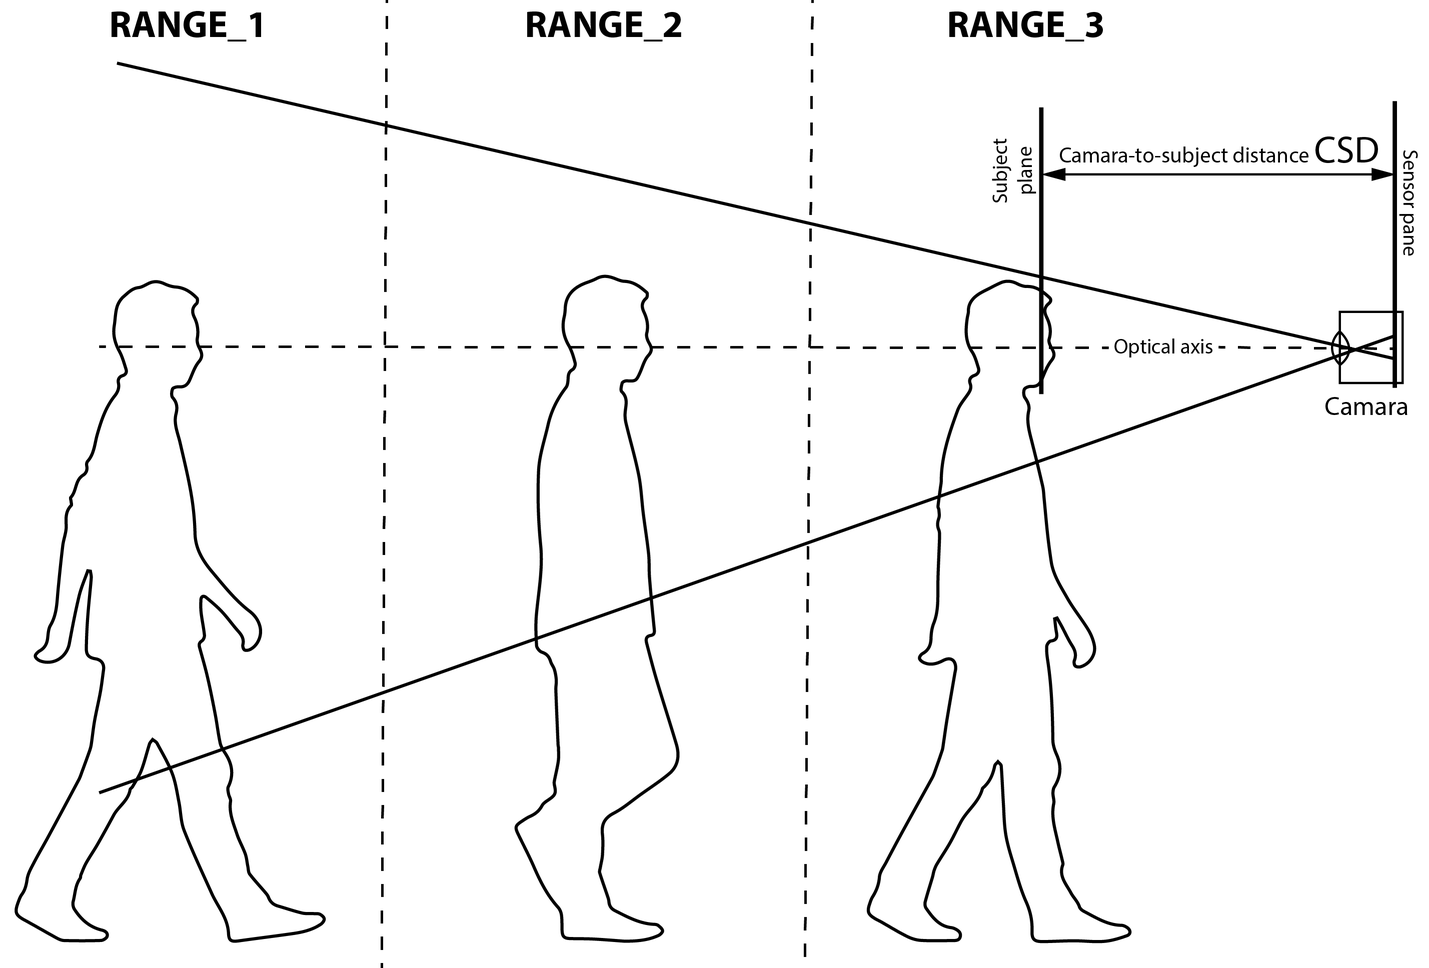
\includegraphics[width=0.8\textwidth]{ch-sistemasABC/images/ch-BBDDs/CAPTURA_ONTHEFLY.png}
     \caption{Esquema del proceso de captura de \textit{FRAV-OnTheFly}.}
     \label{fig:EsquemaCapturaFRAVABCOmTheFly}
\end{figure}

La base de datos de \Gls{FRAV-OnTheFly} incluye 178 sujetos y contiene 1068 vídeos. Estos vídeos tienen 25 fps (fotogramas por segundo) y una resolución de $1,920\times1,080$ píxeles (ver Fig. \ref{fig:fravattackonthefly}).

La base de datos consta de 82 mujeres y 96 hombres. Las edades oscilan entre los 18 y los 67 años, con aproximadamente el $70$ por ciento de los sujetos en el rango de edad de $18$ a $28$ años. La selección de los individuos para la base de datos se hizo de acuerdo con las estadísticas de cruce de fronteras que imitan su distribución. Se construyó una base de datos con estudiantes voluntarios, profesores y personal universitario. Todos los sujetos mantienen su privacidad y, de acuerdo con las normas de protección de datos, se requirió el consentimiento informado de todos los sujetos. La adquisición de buena fe se llevó a cabo durante una semana y después, tras construir los \GLS{PAI} de todos los sujetos, la captura de los vídeos de ataque se realizó en dos días. 

Los vídeos para la base de datos se capturaron en el laboratorio en condiciones de iluminación controlada. Estos vídeos se grabaron con una cámara de alta resolución Sony\textsuperscript{\textregistered}$\alpha6000$ (ver apartado \ref{sec:BBDD-FRAV-Attack}). 

Se enseñó a los sujetos a simular el comportamiento de los viajeros en un cruce de frontera con un sistema \GLS{ABC} de captura dinámica. Así, los sujetos caminan desde 3 metros de la cámara hasta medio metro (ver Fig. \ref{fig:EsquemaCapturaFRAVABCOmTheFly}). Se grabaron seis vídeos diferentes siguiendo este procedimiento (uno por cada tipo de ataque y uno para el \gls{bona-fide}). 

\begin{table}
\centering
\begin{tabular}{|c|c|c|}
\hline
\textbf{Rango} & \textbf{Tamaño imagen} & \textbf{Distancia} \\ \hline
\textbf{Fuera de Rango} & $50\times50$ px & -- \\ \hline
\textbf{Rango-$1$} & $\geq{}$ $50\times50$ px -- \textless{} $150\times150$ px & $\geq{}$ $2$m \\ \hline
\textbf{Rango-$2$} & $\geq{}$ $150\times150$ px -- \textless{} $250\times250$ px & \textless{} $2$m $\geq{}$ $1$m \\ \hline
\textbf{Rango-$3$} & $\geq{}$ $250\times250$ px & \textless{} $1$m \\ \hline
\end{tabular}
\caption{Rangos en los que se clasifican las caras en \Gls{FRAV-OnTheFly} y en \Gls{FRAV-ABC-OnTheFly} atendiendo a la distancia del sujeto al dispositivo, calculada mediante al tamaño de la región de cara detectada.}
\label{tab:facesranges_FRAV_OnTheFly}
\end{table}

Una vez que se capturaron todos los vídeos se realizó un proceso de recuperación de las imágenes faciales. Cada fotograma de los vídeos fue procesado con el algoritmo \textit{\gls{Viola-Jones}} \cite{viola2004robust} para detectar caras. Atendiendo al tamaño de la región detectada, las caras se etiquetaron en un determinado rango. Se consideraron tres rangos (ver Tabla \ref{tab:facesranges_FRAV_OnTheFly}). 

\medskip
\textbf{Rango-1}

Caras detectadas a más de 2 metros del dispositivo, cuya región tiene un tamaño mayor o igual que $50\times50$ píxeles y menor que $150\times150$ píxeles.

\medskip
\textbf{Rango-2}

Caras detectadas a una distancia entre 1 metro y 2 metros del dispositivo, cuya región tiene un tamaño mayor o igual que $150\times150$ píxeles y menor que $250\times250$ píxeles.

\medskip
\textbf{Rango-3}

Caras detectadas a menos de 1 metro del dispositivo, cuya región tiene un tamaño mayor que $250\times250$ píxeles.

\medskip
\textbf{Fuera de rango}

Las caras detectadas con regiones menores a $50\times50$ píxeles se consideraron caras fuera de rango que no pueden ser procesadas. 

\medskip

\begin{table}[ht!]
    \centering
    \begin{tabular}{|l|c|c|c|c|c|c|} \hline
    \multicolumn{7}{|c|}{\rule{0pt}{25pt} \shortstack{\textbf{FRAV-OnTheFly} \\ ($178$ subjects - $1,068$ videos - $120,425$ faces)}} \\ \hline 
    \small{\textbf{Rango}} & \small{\textbf{Bona fide}} & \small{\textbf{Photo}} & \small{\textbf{Video}} & \small{\textbf{Mask}} & \small{\textbf{Mask w/e}} & \small{\textbf{$3$D Mask}} \\ \hline 
    \small{\textbf{Rango-$1$}} & $8,799$ & $8,525$ & $8,330$ & $8,203$ & $8,329$ & $412$ \\ \hline
    \small{\textbf{Rango-$2$}} & $8,837$ & $8,730$ & $8,750$ & $8,335$ & $8,420$ & $441$ \\ \hline
    \small{\textbf{Rango-$3$}} & $8,843$ & $8,603$ & $8,603$ & $8,208$ & $8,225$ & $435$ \\ \hline
    \end{tabular}
    \caption{Número de caras detectadas en los vídeos de la base de datos \gls{FRAV-OnTheFly}.}
    \label{tab:faces-FRAV-OnTheFly}
\end{table}

Finalmente, la información de la base de datos es almacenada para los tres rangos definidos (Ver Tabla \ref{tab:faces-FRAV-OnTheFly}). Nótese que hay diferentes cantidades de fotogramas con caras porque a veces una cara no puede ser detectada en todos los fotogramas de la secuencia.


%%%%%%%%%%%%%%%%%%% FRAV ABC ONTHEFLAY CAPTURADA EN ABC %%%%%%%%%%%%%%%
\subsection{\textit{FRAV-ABC-OnTheFly}: ABC en frontera real}\label{subsec:BBDD-FRAV-ABC-OnTheFly}

\begin{figure}[h!]
    \centering
    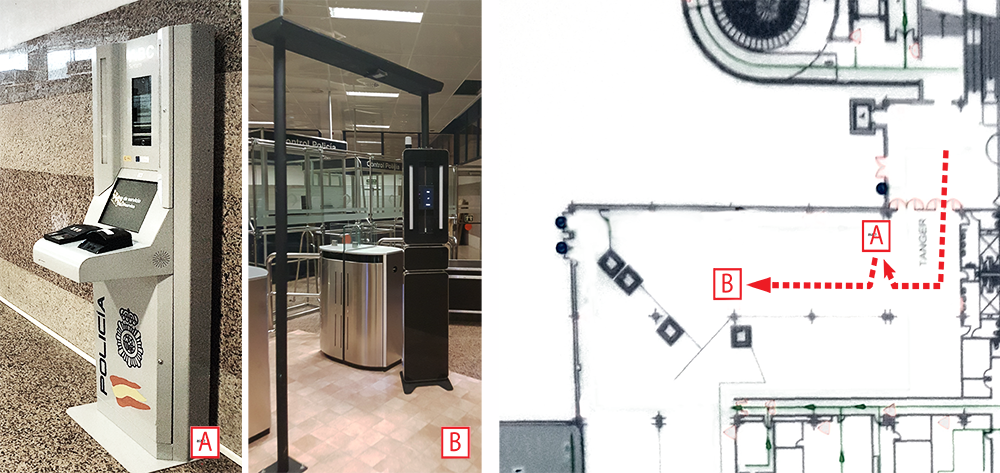
\includegraphics[width=1\textwidth]{ch-sistemasABC/images/ch-onthefly/realDevices.png}
    \caption{Escenario real con los dispositivos \gls{e-kiosk} y \gls{e-gate}.}
    \label{fig:realdevices}
\end{figure}

La base de datos \Gls{FRAV-ABC-OnTheFly} se capturó en un sistema \GLS{ABC} \textit{<<Segregated Two Step>>}\footnote{\Gls{FRAV-ABC-OnTheFly} se capturó durante la implantación de los sistemas \GLS{ABC} piloto del Proyecto Europeo \GLS{ABC4EU} \cite{ABC4EUOnline} en el puerto marítimo de Algeciras (España). Este puerto es una frontera del área de \textit{\Gls{Schengen}}, siendo un importante punto de entrada y salida para viajeros del norte de África.} con dos dispositivos: un \gls{e-kiosk} donde se realizaba la etapa \GLS{RTP} y un \gls{e-gate} para la etapa de \GLS{EES} (ver Fig. \ref{fig:realdevices}). Los viajeros se registraban en el \gls{e-kiosk}, mostrando su documentación y posteriormente se dirigían a la \gls{e-gate} para completar el cruce. La captura en el \gls{e-kiosk} se realizaba de forma estática, el viajero debe detenerse ante el dispositivo para que su identidad se verifique con la almacenada en sus documentos. Sin embargo en la \gls{e-gate} la captura es dinámica y la verificación con alguna de identidades registradas se realiza mientras que el viajero se aproxima a la puerta.
% (la arquitectura \Gls{FlyPAD} Para esta captura dinámica es para la que se propone  presentada en el capitulo \ref{ch:ABC_OnTheFly}.

\Gls{FRAV-ABC-OnTheFly} incluye 10 sujetos, 5 mujeres y 5 hombres, de edades comprendidas entre los 22 y los 56 años. Al igual que en \Gls{FRAV-OnTheFly} se grabaron vídeos de $1920\times1080$ píxeles a 25 fps, Con cada sujeto se grabó un vídeo \gls{bona-fide} aproximándose a la puerta y 5 vídeos de ataque con diferentes \GLS{PAI}.

\begin{table}[ht!]
\centering
\begin{tabular}{|l|c|c|c|c|c|c|} \hline
\multicolumn{7}{|c|}{\rule{0pt}{25pt} \shortstack{\textbf{FRAV-ABC-OnTheFly} \\ ($10$ subjects - $60$ videos - $7,200$ faces)}} \\ \hline
\small{\textbf{Range}} & \small{\textbf{Bona fide}} & \small{\textbf{Photo}} & \small{\textbf{Video}} & \small{\textbf{Mask}} & \small{\textbf{Mask w/e}} & \small{\textbf{$3$D Mask}} \\ \hline 
\small{\textbf{Range-$1$}} & $440$ & $402$ & $318$ & $350$ & $347$ & $408$ \\ \hline
\small{\textbf{Range-$2$}} & $481$ & $411$ & $421$ & $417$ & $428$ & $423$ \\ \hline
\small{\textbf{Range-$3$}} & $403$ & $383$ & $370$ & $403$ & $408$ & $387$ \\ \hline
\end{tabular}
\caption{Número de caras detectadas en los vídeos de la base de datos \Gls{FRAV-ABC-OnTheFly}.}
\label{tab:faces-FRAV-ABC-OnTheFly}
\end{table}

Una vez que se capturaron todos los vídeos se realizó un proceso de recuperación de las imágenes faciales y una clasificación por rangos, atendiendo a la  distancia del sujeto al dispositivo. Los rangos considerados son los mismos que en \Gls{FRAV-OnTheFly} (ver apartado \ref{subsec:BBDD-FRAV-OnTheFly}) y el número total de caras detectadas en cada rango se pude ver en la tabla \ref{tab:faces-FRAV-ABC-OnTheFly}.

\begin{landscape}
\begin{figure}
    \centering
    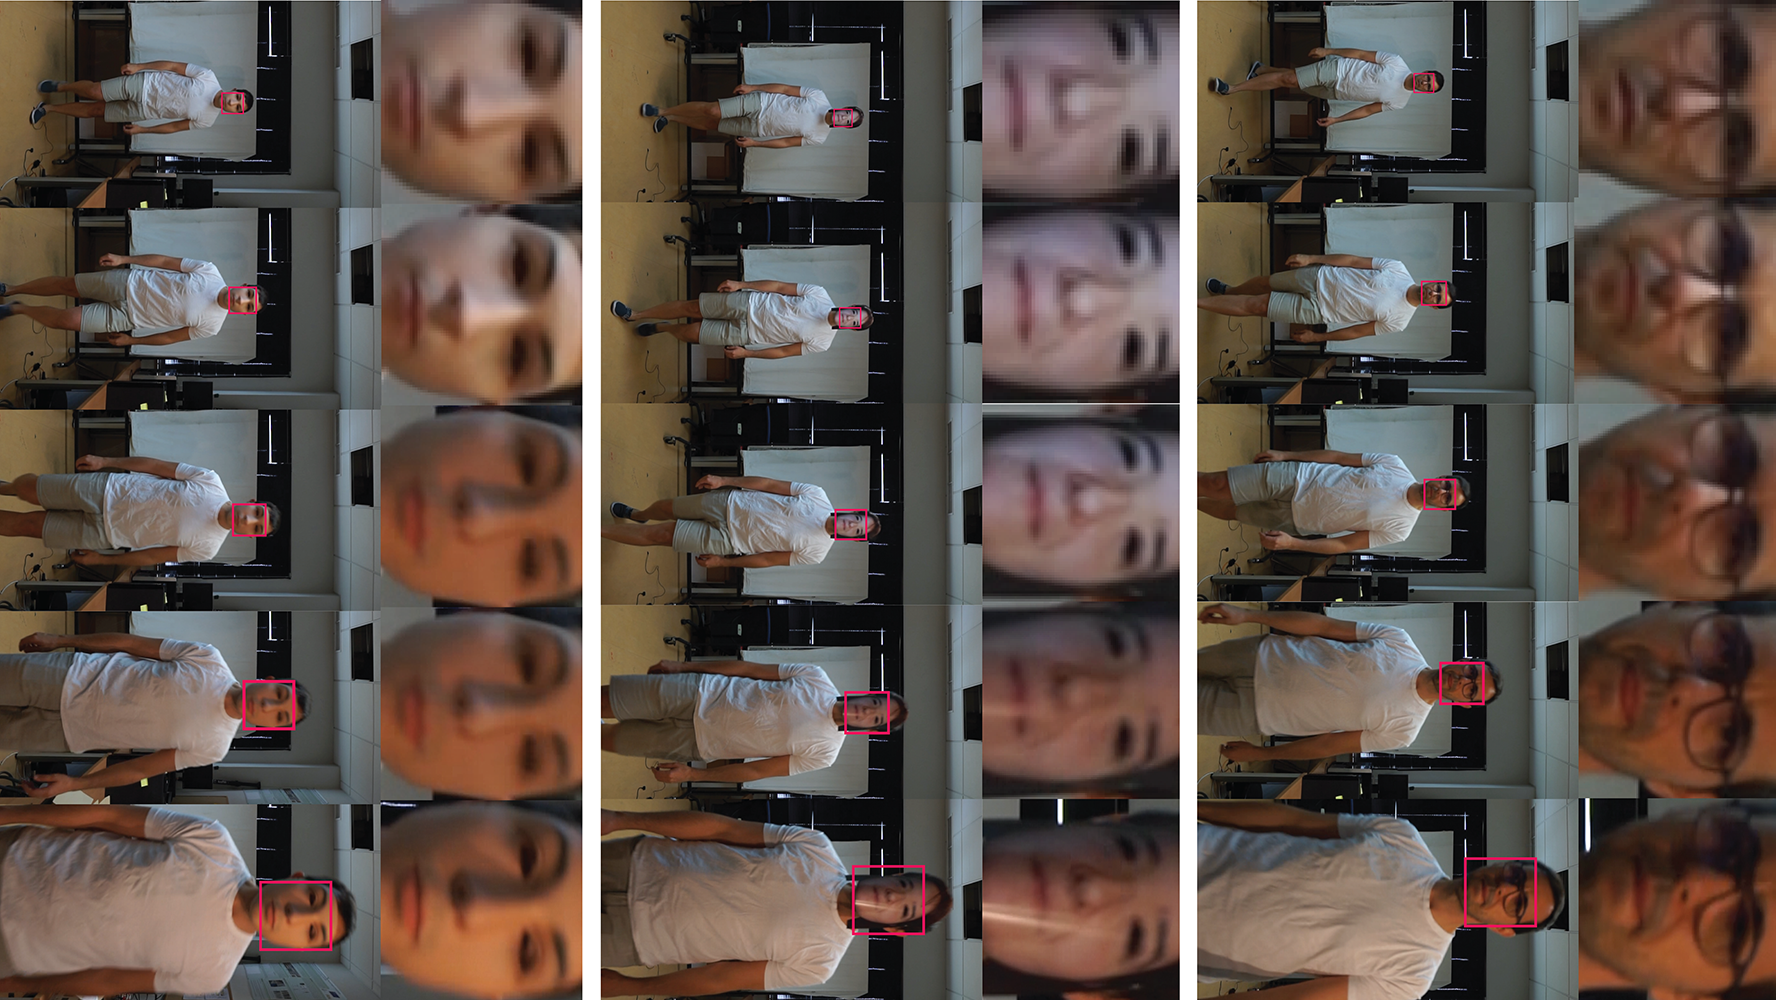
\includegraphics[scale=1.5]{ch-sistemasABC/images/ch-BBDDs/FRAVAttackOnTheFly.png}
    \caption{Capturas de vídeos almacenados en la base de datos \Gls{FRAV-OnTheFly}.}
    \label{fig:fravattackonthefly}
\end{figure}
\end{landscape}

%%%%%%%%%%%%%% FRAV ABC MORPHING  %%%%%%%%%%%%%%%%%%%%%%%%%%%%%%%%%%%%%%% 
\section{Bases de datos para MAD}\label{sec:BBDD_Morphing}

En esta sección se presenta la base de datos \Gls{FRAV-Morphing} construida para investigaciones sobre ataques de presentación de tipo \gls{morphing} \Gls{FRAV-Morphing}. Los ataques se han creado fusionando las imágenes \gls{chip} de los sujetos de la base de datos \Gls{FRAV-ABC} (ver sección \ref{sec:BBDD-ABC}), construyendo imágenes \gls{chip morphing} mediante un método automático descrito en el apartado \ref{subsec:MorphingMethods}.

de la publicación \cite{ortega2020border}, descrita en detalle en el Capítulo \ref{ch:morphing}.  

En el apartado \ref{subsec:FRAV-Morphing} se explica cómo se ha estructurado la base de datos en varios subconjuntos para entrenamiento, validación y test, evitando mezclar sujetos entre conjuntos.

En el apartado \ref{subsec:BBDD_MorphingPrintScan} se explica como se imprimieron y se escanearon para acercar los datos a la problemática real que se produce en la construye un documento de viaje.

%%%%%%%%% METODO MORPHING  %%%%%%%%%%%
\subsection{Método \textit{morphing}}\label{subsec:MorphingMethods}

\begin{figure}[ht]
     \centering
     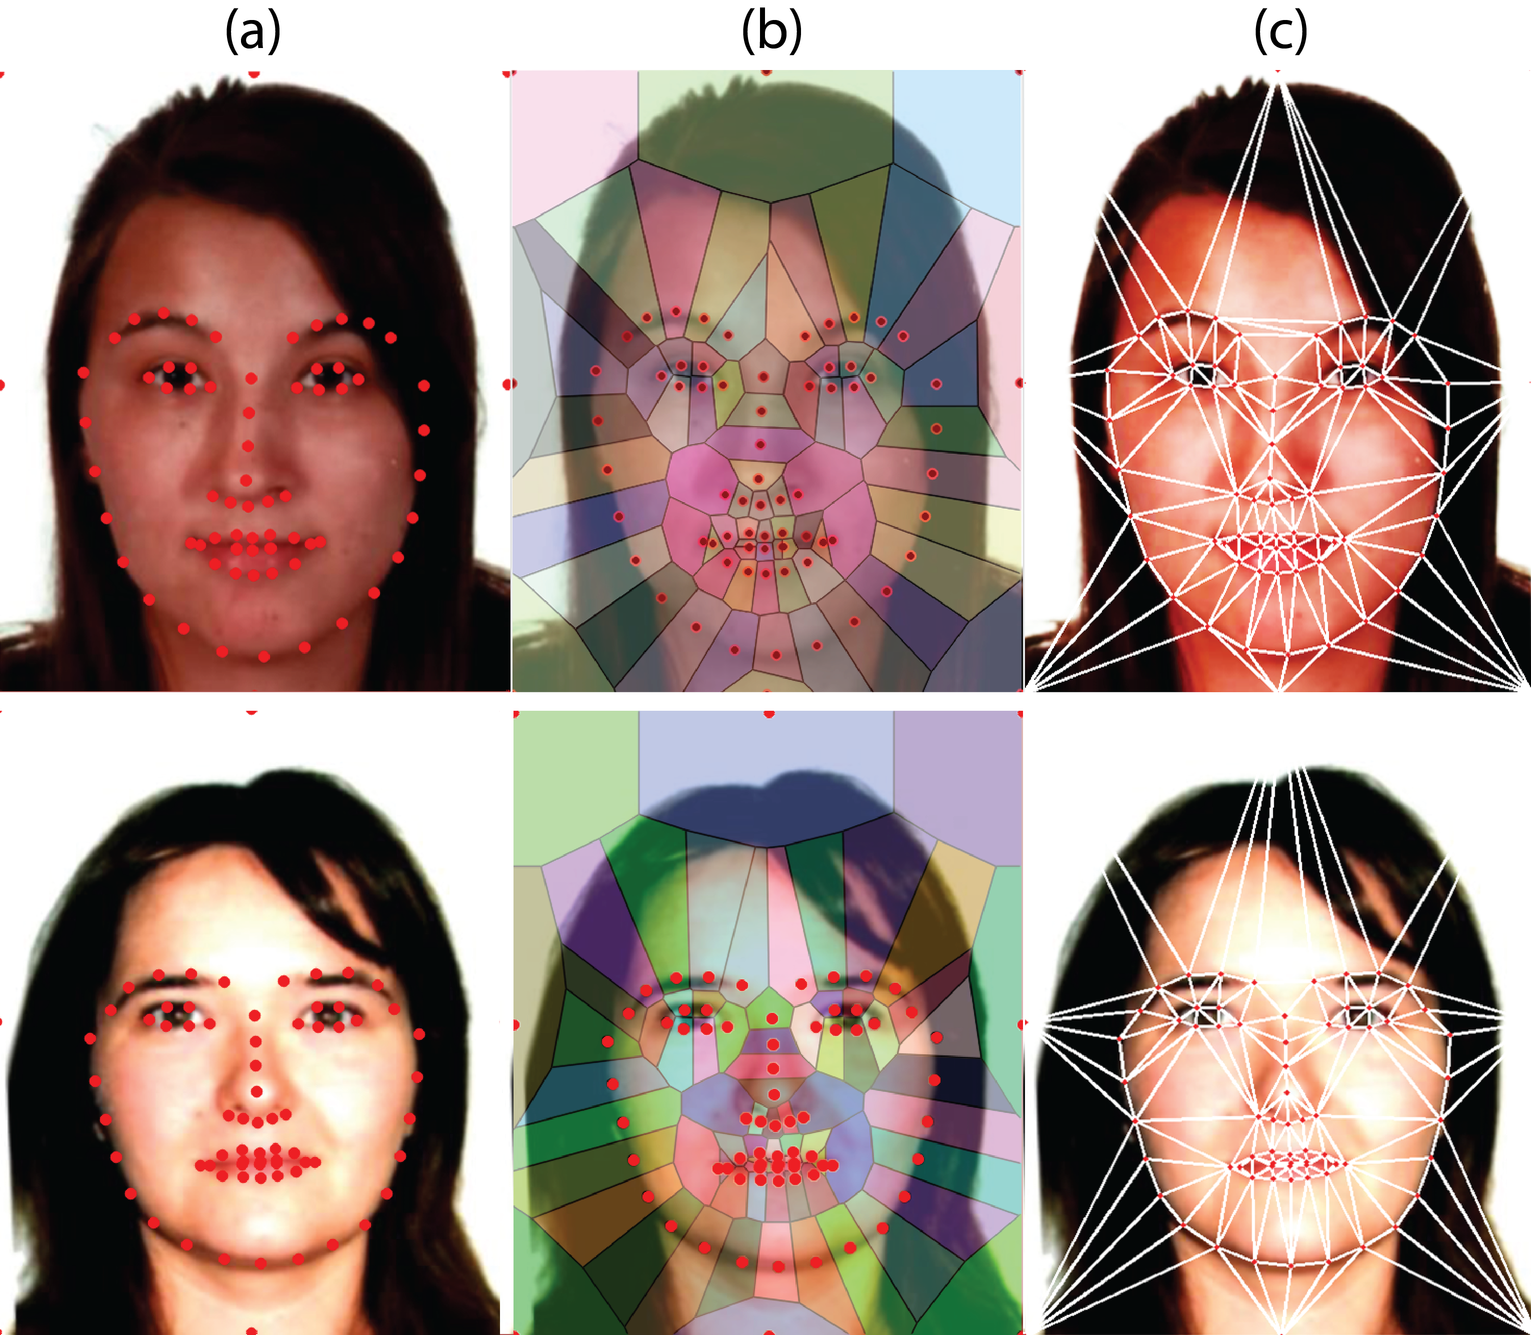
\includegraphics[width=0.8\textwidth]{ch-sistemasABC/images/ch-morphing/TRIANGULACION-CHIP-BEA-CRISTINA.png}
     \caption{(a) \textit{Detección de Landmark faciales}, (b) \textit{Calculo de Delaunay} y (c) \textit{Triangulación Voronoi}.}
     \label{fig:LandmarckDVTriangualtion}
\end{figure}

\begin{figure}[ht]
     \centering
     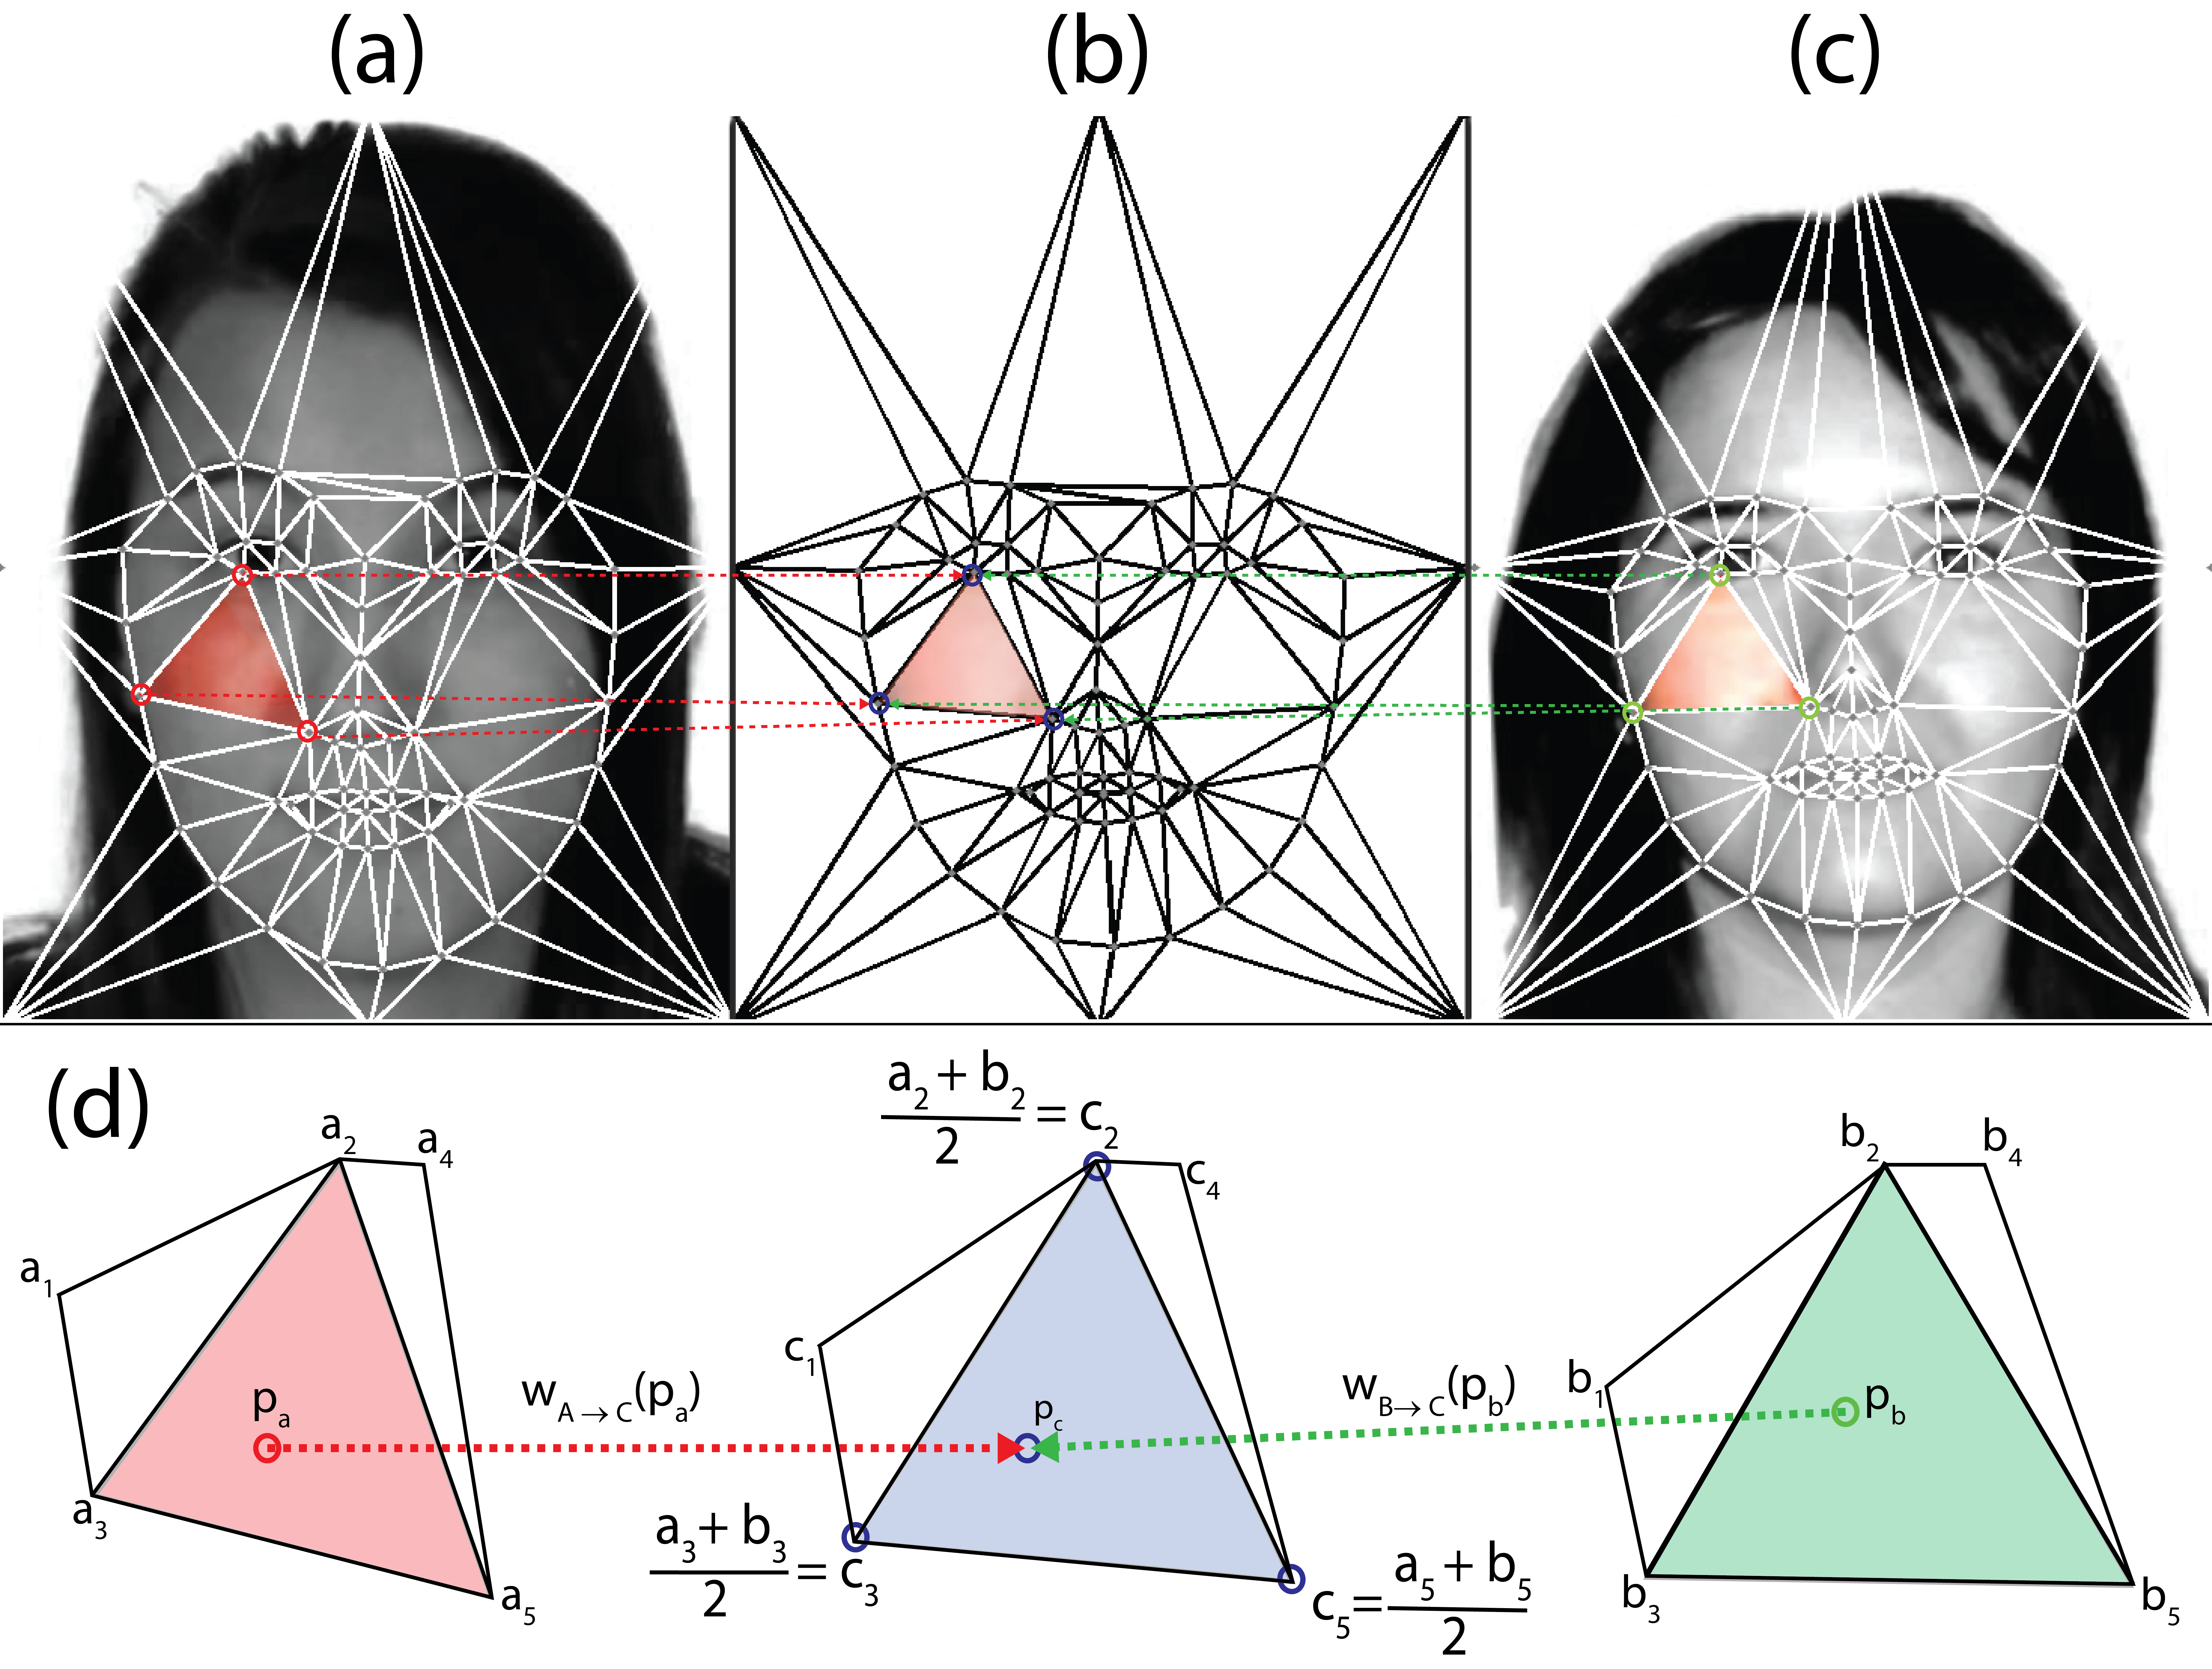
\includegraphics[width=0.8\textwidth]{ch-sistemasABC/images/ch-morphing/TriangulacionFusion_CristinaBea_COMPACTA.png}
     \caption{Warping the morphed target image and blending each source triangle that contained pixels.}
     \label{fig:Triangulación}
\end{figure}

\begin{figure}[ht]
     \centering
     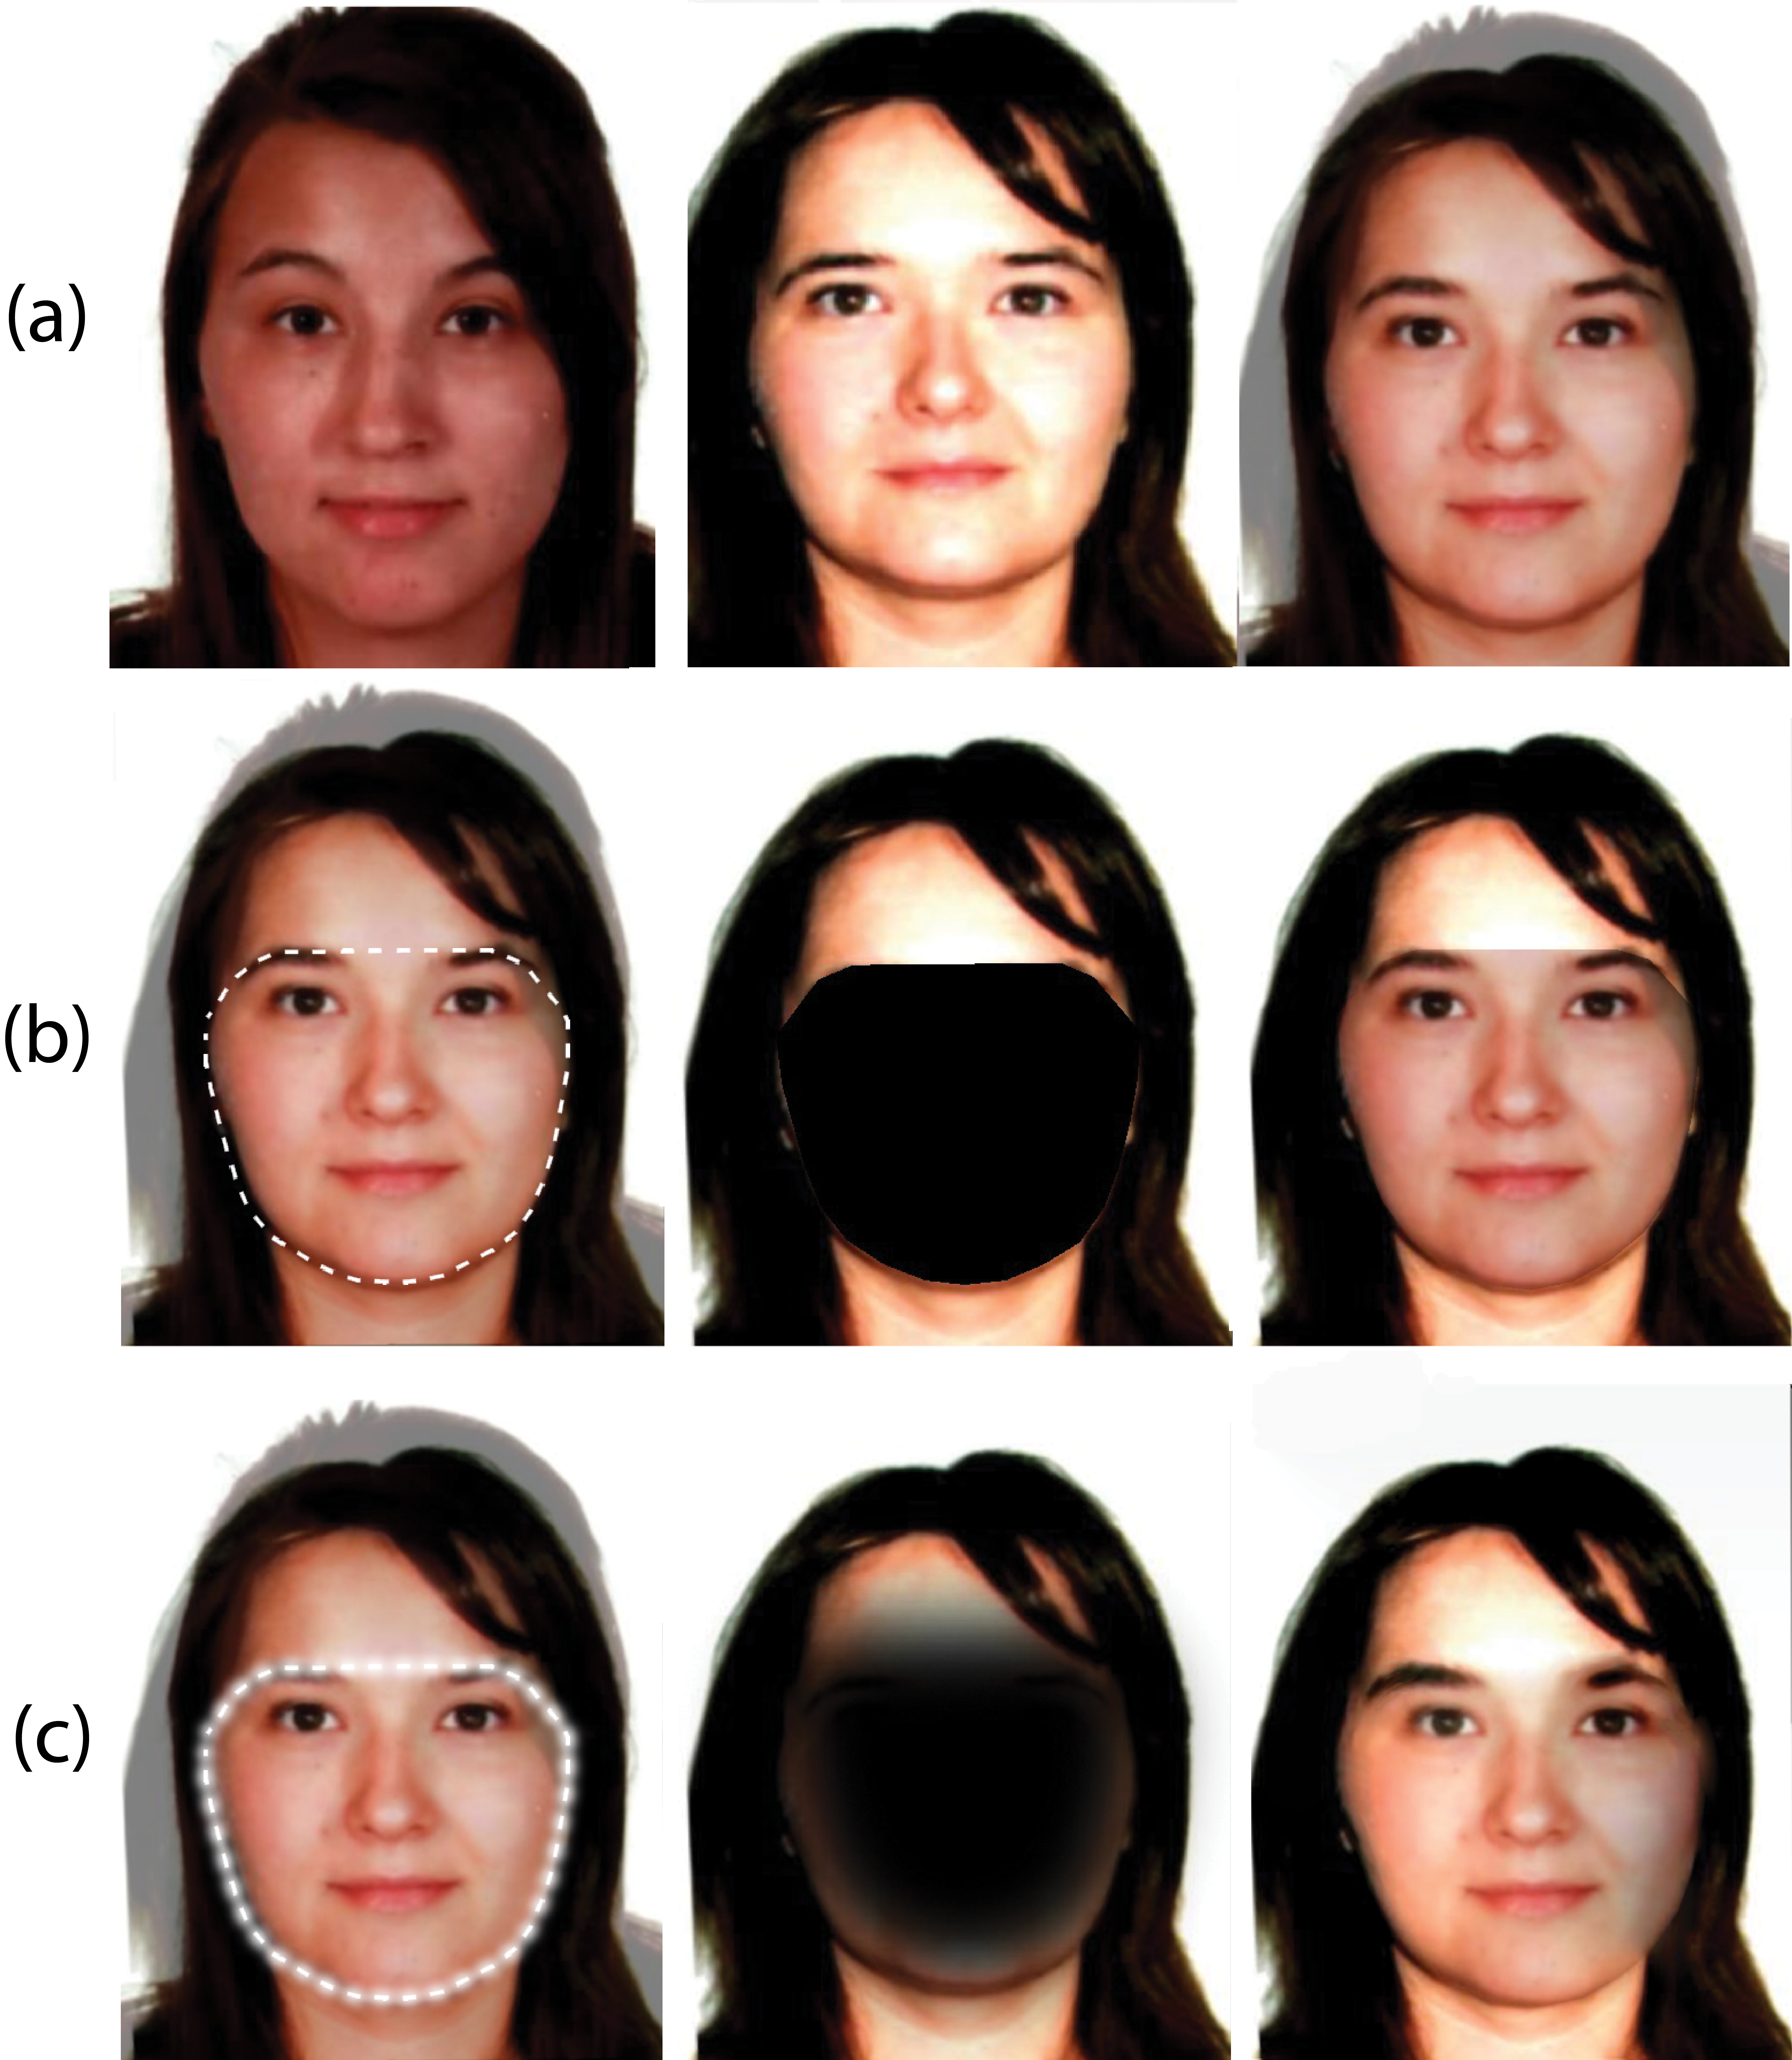
\includegraphics[width=0.8\textwidth]{ch-sistemasABC/images/ch-morphing/MorphingEnhanceMask_COMPACTA.png}
     \caption{(a)Average image, (b) Clipping and replacing the  face region and (c) the fuzzy mask to enhance the result and cropping source image.}
     \label{fig:Enhancement}
\end{figure}

% \begin{figure}[ht]
%     \centering
%     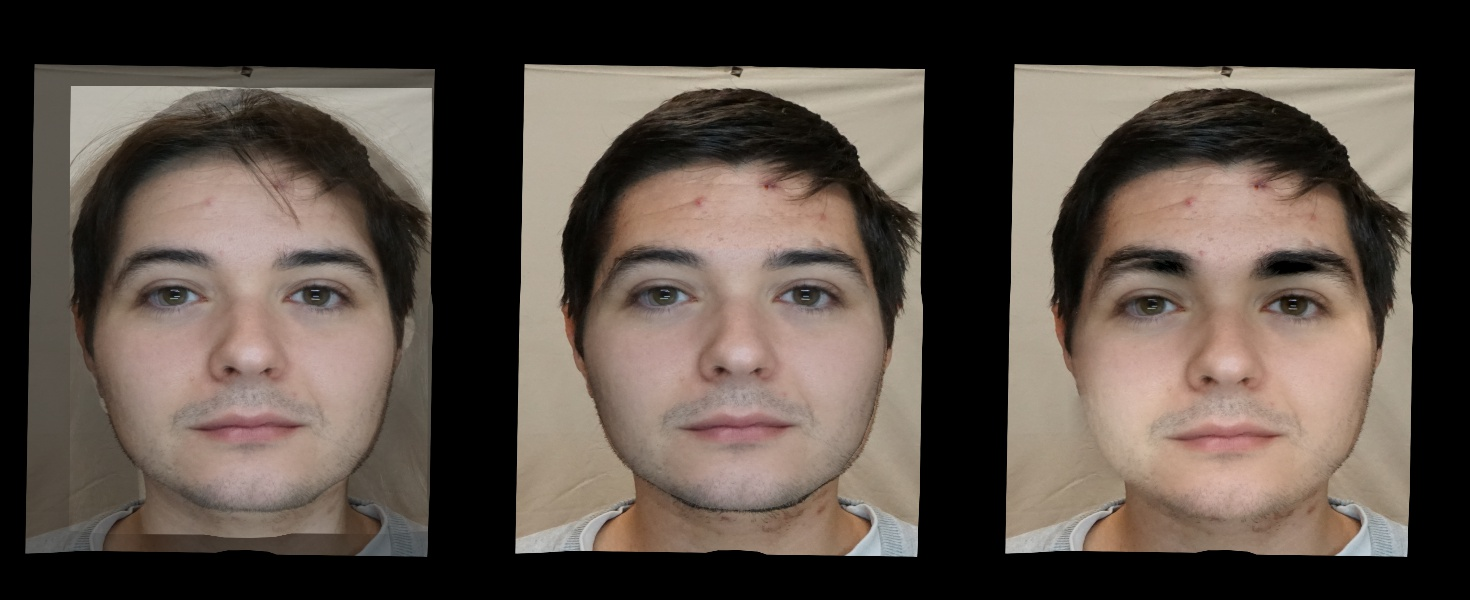
\includegraphics[width=\textwidth]{ch-sistemasABC/images/ch-morphing/old/coreccion_mophings.jpg}
%     \caption{Corrección del \textit{morphing}.}
%     \label{fig:morphing_correccion}
% \end{figure}

% \begin{figure}[ht]
%     \centering
%     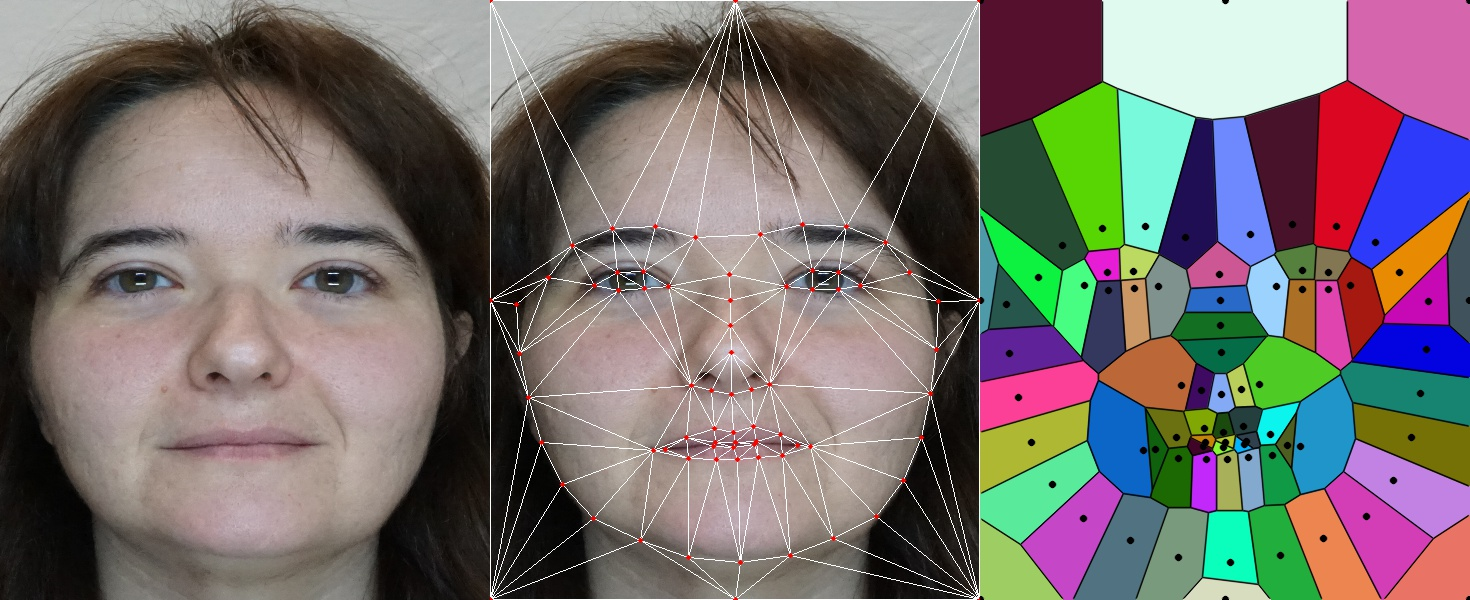
\includegraphics[width=\textwidth]{ch-sistemasABC/images/ch-morphing/old/delaunay-voronoy.jpg}
%     \caption{Triangulación Delaunay-Voronoi.}
%     \label{fig:morphing_delaunay_voronoi}
% \end{figure}

% \begin{figure}[ht]
%     \centering
%     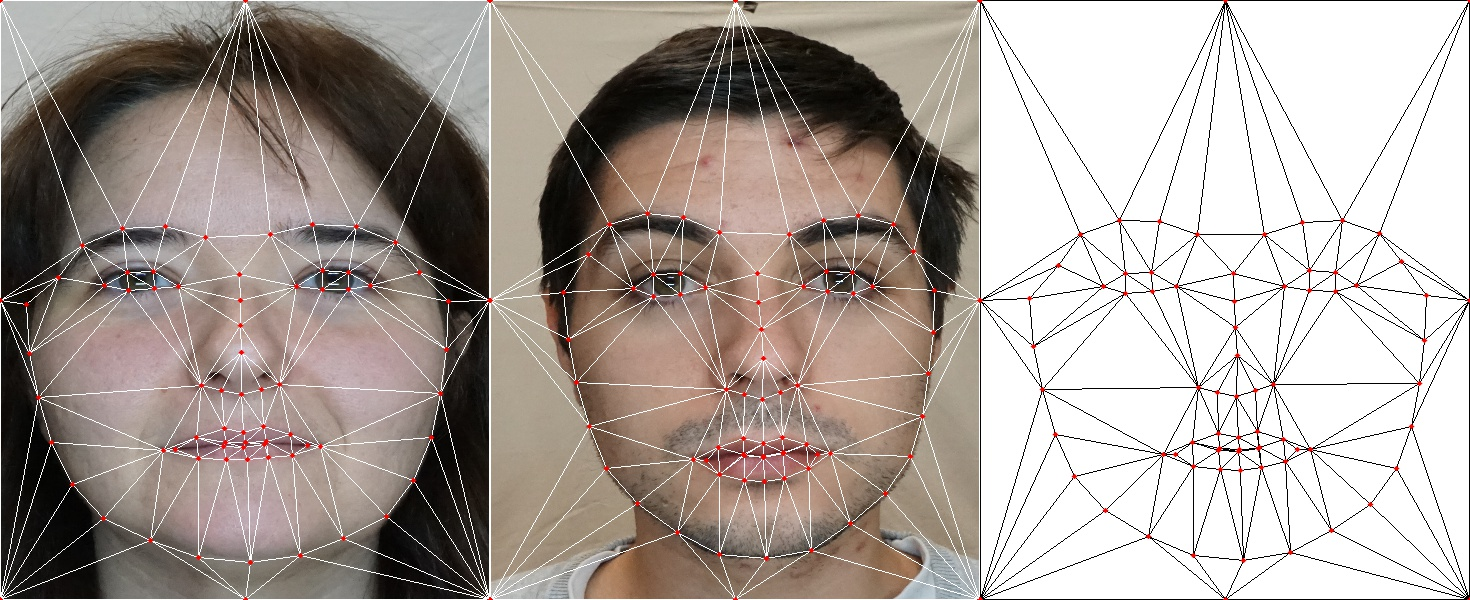
\includegraphics[width=\textwidth]{ch-sistemasABC/images/ch-morphing/old/triangulationImage.jpg}
%     \caption{Triangulación del \textit{morphing}.}
%     \label{fig:morphing_triangulacion}
% \end{figure}

Actualmente, es posible encontrar herramientas de software comercial para la construcción de imágenes \gls{morphing} de alta calidad (\cite{FantaMorphOnline}, \cite{MorpheusOnline}, \cite{MorphThingOnline}, \cite{NukeOnline}, \cite{SilhouetteFXOnline}, \cite{GimpOnline}, \cite{FaceMorpherOnline}, \cite{WinMorphOnline}), pero todas ellas, en mayor o menor medida, requieren procesos manuales. Cuando se necesita un gran número de imágenes hay que buscar un proceso automático. El algoritmo presentado en \cite{ferrara2017face}, \cite{scherhag2019face} permite esta automatización del proceso. 

Esta sección describe el proceso \gls{morphing} empleado para la construcción de los distintos conjuntos de la base de datos \Gls{FRAV-Morphing}. El proceso propuesto se divide en dos etapas: Una primera de fusión de las identidades que mezcla las dos imágenes y una segunda de corrección y mejora del resultado final que consigue una imagen más realista.

\medskip
\textbf{Fusión de identidades}
\medskip

La construcción del \textit{morphing} se realiza en tres de pasos: Detección de punto de referencia, triangulación y mezcla.

\begin{enumerate}

\item 
Dadas las dos imágenes a fusionar en cada una de ellas se detectan $76$ puntos de referencia que posteriormente ayudarán en su triangulación: $68$ \textit{\glspl{landmark}} faciales. detectados mediante el algoritmo propuesto por \textit{Kazemi} y \textit{Sullivan} \cite{kazemi2014one} (implementado en \Gls{Dlib} \cite{dlibOnline}) y ocho puntos que forma parte del borde de la imagen (las esquinas y los puntos medios de cada lado)

\item 
con los puntos de referencia detectados se realiza una triangulación de las imágenes con el algoritmo \textit{Delaunay-Voronoi} (\GLS{DVT} \cite{lokhande2013morphing}) (ver Figura \ref{fig:LandmarckDVTriangualtion}, que consiste en unión de los puntos de referencia (con camino \textit{Delaunay} mínimo) de los puntos de regiones de \textit{Voronoi} colindantes (ver Fig. \ref{fig:LandmarckDVTriangualtion} (b) y (c)). Como la triangulación se realiza en las dos imágenes a fusionar cada triangulo en una imagen  tiene un triángulo homólogo en la otra imagen (Fig. \ref{fig:Triangulación}).

\item 
Cada par de triángulos homólogos se deforman y se mezclan componiendo una nueva imagen que es la imagen promedio, este proceso de deformación y mezcla se conoce como \textit{warping} \cite{wu2011face}, \cite{jassim2018automatic}, \cite{hildebrandt2017benchmarking} (ver Fig. \ref{fig:Triangulación}). Los vértices de cada nuevo triangulo son los puntos medios de los vértices correspondientes de los triángulos a deformar y lo \textit{pixels} contenidos se fusionan atendiendo a un factor de mezcla (habitualmente al $50$\%). 

\end{enumerate}

\medskip
\textbf{Corrección y mejora de la fusión}
\medskip


La imagen promedio tiene demasiados artefactos (\textit{ghost artifacts}), especialmente en las regiones periféricas y resulta muy detectable visualmente como ataque de presentación (ver Fig. \ref{fig:Enhancement} (a)). Para mejorar el resultado final de la fusión y obtener una apariencia más realista se puede retocar la imagen manualmente \cite{ferrara2014magic} o aplicar algunos ajustes automáticos \cite{ferrara2017face}:

\begin{enumerate}
\item 
Una mejora consiste en: detectar los \textit{\glspl{landmark}} faciales en la imagen promedio, calcular su envolvente convexa (forma convexa que circunscribe todos los puntos), recortar la envolvente convexa en la imagen promedio y pegar el recorte en alguna de las dos imágenes origen, eliminado así, el efecto de doble imagen (var Fig. {\ref{fig:Enhancement} (b)}). 

\item 
Cuando las imágenes a fusionar tienen diferentes condiciones de iluminación, color de piel o pose el recorte resulta demasiado apreciable. Para que el recorte no se tan duro se aplica una máscara difusa. Utilizando. por ejemplo, la técnica \textit{Poisson Merge} \cite{perez2003poisson} de edición de imágenes, se consigue una fusión más suave (ver Fig. \ref{fig:Enhancement} (c)).
\end{enumerate}

Estas mejoras, evitan los efectos fantasma y los cambios abruptos en la textura y el color de la piel, lo que hace más difícil el proceso de detección. Aunque el \GLS{MAD} descrito en la Sección \ref{sec:de-morphingApproach} no depende del proceso de construcción del \gls{morphing}.

%%%%%%%%% FRAV ABC MORPHING  %%%%%%%%%%%
\subsection{\textit{FRAV-Morphing}}\label{subsec:FRAV-Morphing}

En esta sección se describe en una base de datos para investigaciones sobre ataques \gls{morphing} \Gls{FRAV-Morphing}, construida a partir de los datos de \Gls{FRAV-ABC} (ver Sección \ref{subsec:FRAV-ABC}) y \textit{dividida en tres conjuntos}. Con los sujetos de \Gls{FRAV-ABC} se han creado dos conjuntos de datos $175$ sujetos (aprox. el $15$\% del total) para construir \Gls{FRAV-Morphing-Test} y con los $1000$ sujetos restantes $700$ se han reservado para entrenamiento (\Gls{FRAV-Morphing-Train}) y $300$ para la validación (\Gls{FRAV-Morphing-Val})
($70$-$30$\% como se recomienda en \cite{deepLearningBook}). La división se ha realizado a nivel sujeto para evitar que se mezclen identidades entre los tres conjuntos.

\begin{table}[ht!]
    \centering
    \begin{tabular}{|l|c|c|c|c|} \hline
    \multicolumn{5}{|c|}{\rule{0pt}{25pt} \shortstack{\textbf{FRAV-Morphing} \\ ($1185$ subjects)}} \\ \hline 
    &  &  & \small{\gls{chip}}  & \small{\gls{chip}} \\ 
    \small{\textbf{Bases de datos \gls{morphing}}} & \small{\textbf{Type}} & \small{\gls{vivo}} & \small{\textbf{Bona fide}} & \small{\textbf{\Gls{morphing}}}  \\ \hline 
    \small{\textbf{\gls{FRAV-Morphing-Train}}} & Digital & $700$ & $700$ & $489300$ \\ \hline
    \small{\textbf{\gls{FRAV-Morphing-Val}}} & Digital & $300$ & $300$ & $89700$ \\ \hline
    \small{\textbf{\gls{FRAV-Morphing-Test}}} & Digital & $185$ & $185$ & $34040$ \\ \hline
    \small{\textbf{\gls{FRAV-Morphing-Test-PS-300}}} & P\&S & $12$ & $12$ & $144$ \\ \hline
    \small{\textbf{\gls{FRAV-Morphing-Test-PS-150}}} &  P\&S & $12$ & $12$ & $144$ \\ \hline
    \end{tabular}
    \caption{Información de las bases de datos de \Gls{morphing}.}
    \label{tab:BASES_DE_DATOS_ORPHING}
\end{table}

Entre los sujetos de cada conjunto con las imágenes \textit{<<\gls{chip}>>} se han construido imágenes \gls{morphing}, fusionando todos con todos, menos consigo mismo, sin tener en cuenta factores de semejanza entre sujetos, como la edad, la raza o el sexo ya que el interés se centra es entrenar sistemas automáticos más que en el aspecto visual perceptible del resultado. Por ejemplo en \Gls{FRAV-Morphing-Test} con $700$ sujetos, se han construido $489300$ imágenes de \gls{morphing}. En la Tabla \ref{tab:BASES_DE_DATOS_ORPHING} se pude ver el contenido de cada uno de los conjuntos, el numero de imágenes \gls{vivo}, de imágenes \gls{chip} y de \gls{morphing} construidos.

%%%%%%%%%%%%%%%% FRAV ABC MORPHING P&S %%%%%%%%%%%%%%%%%%%%%%%%%%%%%%%%% 
\subsection{\textit{FRAV-Morphig} impresa y escaneada.}\label{subsec:BBDD_MorphingPrintScan}

\begin{figure}[ht]
     \centering
     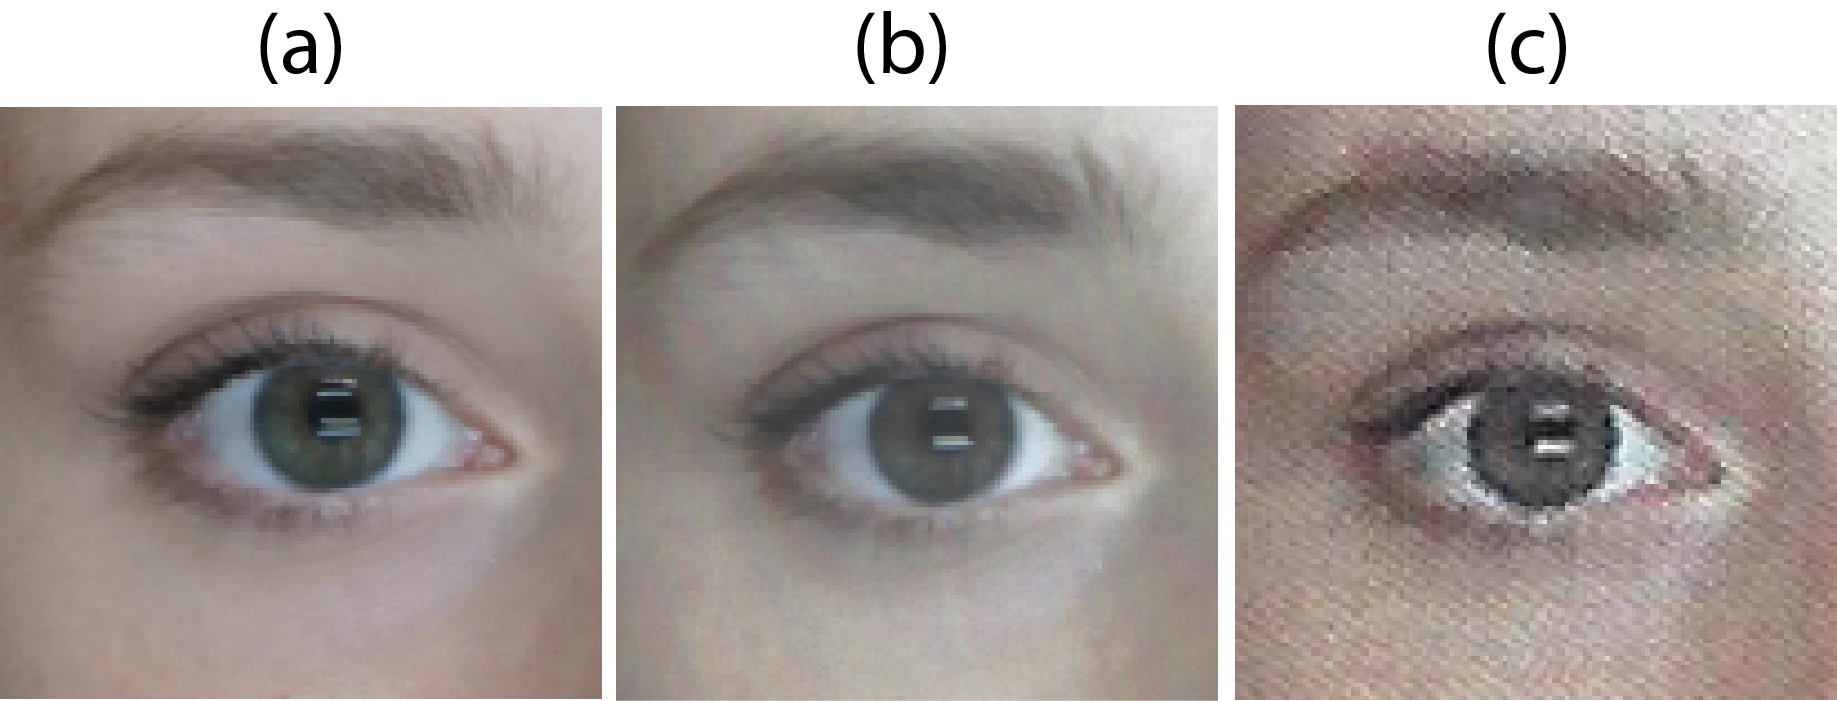
\includegraphics[width=0.8\textwidth]{ch-sistemasABC/images/ch-morphing/CalidadImpresas.png}
     \caption{(a) Calidad delas imágenes \Gls{FRAV-Morphing-Test}. (b) Calidad de las imágenes \Gls{FRAV-Morphing-Test-PS-300}. (c) Calidad de imágenes \Gls{FRAV-Morphing-Test-PS-150}.}
     \label{fig:NOISE_PrintScan}
\end{figure}

El proceso habitual para la expedición de pasaportes consiste en escanear una fotografía, previamente impresa, del viajero. Esto hace que la imagen almacenada finalmente el \text{<<\gls{chip}>>} del \gls{eMRTD} tenga una degradación que influye a la hora de detectar ciertos ataques, especialmente el \gls{morphing} (ver Fig. \ref{fig:NOISE_PrintScan}). Para evaluar la eficacia de los \GLS{MAD} en circunstancias reales se han construido dos conjuntos de datos con imágenes impresas y escaneadas.

Se seleccionan los $12$ sujetos de \Gls{FRAV-Morphing-Test} que consiguen un mejor \textit{score} de verificación con \gls{FaceNet} \cite{schroff2015facenet}, entre sus imágenes \gls{vivo} y los \gls{chip} \gls{morphing}. Es decir, aquellos que mejor consiguen engañar a un sistema reconocimiento facial.

Las $12$ imágenes \textit{<<\gls{chip}>> \gls{bona-fide}} y las $144$ imágenes \gls{chip} \gls{morphing} de los usuarios seleccionados se han impreso a $300$ \gls{DPI} con una impresora \textit{LaserJet} a color y a continuación se han escaneado para construir un nuevo conjunto de datos (\Gls{FRAV-Morphing-Test-PS-300}). También se repite el proceso de impresión y escaneado, esta vez a $150$ \gls{DPI} para construir \Gls{FRAV-Morphing-Test-PS-150}. (Ver contenido de las bases de datos \Gls{FRAV-Morphing-Test-PS-300} y \Gls{FRAV-Morphing-Test-PS-150} en la Tabla. \ref{tab:BASES_DE_DATOS_ORPHING}).